%=======================================================================
% Wave-Corrected Caustics over Photon Splatting
% IEEEtran journal edition. The body is shared with docs/paper/.
% Compile: python tools/build_paper_ieee.py
%=======================================================================
\documentclass[journal]{IEEEtran}

\usepackage[T1]{fontenc}
\usepackage[utf8]{inputenc}
\usepackage{cite}
\usepackage{amsmath}
\usepackage{amssymb}
\usepackage{amsthm}
\usepackage{booktabs}
\usepackage{multirow}
\usepackage{array}
\usepackage{siunitx}
\usepackage{algorithm}
\usepackage{algpseudocode}
\usepackage{xcolor}
\usepackage{url}
\usepackage{graphicx}
\graphicspath{{../paper/figures/}{../paper/}}

\setcounter{secnumdepth}{2}
\sisetup{detect-all,group-separator={,},group-minimum-digits=4}

\theoremstyle{plain}
\newtheorem{theoremcounter}{Theorem}
\newtheorem{lemma}[theoremcounter]{Lemma}
\newtheorem{corollary}[theoremcounter]{Corollary}
\newtheorem{proposition}[theoremcounter]{Proposition}
\theoremstyle{definition}
\newtheorem{definition}[theoremcounter]{Definition}
\theoremstyle{remark}
\newtheorem{remark}[theoremcounter]{Remark}
\newtheorem{assumption}[theoremcounter]{Assumption}

\newcommand{\Hm}{\mathbf{H}}
\newcommand{\Jm}{J_{\Hm}}
\newcommand{\fold}{\mathcal{F}}
\newcommand{\recv}{\Omega}
\newcommand{\dir}{\hat{\mathbf{s}}}
\newcommand{\nrm}{\mathbf{n}}
\newcommand{\trn}{\hat{\mathbf{t}}}
\newcommand{\Ai}{\operatorname{Ai}}
\newcommand{\detJ}{\det \Jm}
\newcommand{\dd}{\mathrm{d}}
\newcommand{\order}[1]{\mathcal{O}\!\left(#1\right)}
\DeclareMathOperator{\sinc}{sinc}

% IEEEtran places a table* caption flush against the table body. The commands
% table (Table XIV) is the one table whose caption follows the tabular, and it
% touched the bottom rule; this supplies the missing gap.
\newcommand{\tablecapgap}{\vspace{1em}}

\renewcommand{\topfraction}{0.92}
\renewcommand{\bottomfraction}{0.5}
\renewcommand{\textfraction}{0.06}
\renewcommand{\floatpagefraction}{0.7}
\renewcommand{\dbltopfraction}{0.92}
\renewcommand{\dblfloatpagefraction}{0.7}
\setlength{\parskip}{0pt}

\markboth{IEEE Transactions on Visualization and Computer Graphics}%
{Chetri and Chauhan: Wave-Corrected Caustics over Photon Splatting}

\begin{document}

%-----------------------------------------------------------------------
% IEEE title, author, abstract, keywords.
% The abstract is the CGF abstract verbatim; the parity check compares the
% whitespace-normalised text of the two abstracts and fails on any drift.
%-----------------------------------------------------------------------
\title{Wave-Corrected Caustics over Photon Splatting: Fold Kinematics,
a Band-Local Airy Correction, and a Comparative Evaluation Against
Production Solvers}

\author{A.~Chetri and Vaishali~Chauhan%
\thanks{A.~Chetri and V.~Chauhan are with Manipal University Jaipur, Jaipur, Rajasthan 303007, India (e-mail: ankit.byte.404@gmail.com).}%
\thanks{A.~Chetri is the corresponding author (GitHub: \texttt{Debyte404}, ORCID: 0009-0004-2672-3503).}%
\thanks{V.~Chauhan is with Manipal University Jaipur (ORCID: 0000-0003-0549-4727).}%
}

\maketitle

\begin{abstract}
We describe a hybrid caustic estimator. Photon splatting and path-traced caustics both diverge at the fold. We treat that as a model property, not a discretisation error. A geometric quadrature carries the image; a wave-optical correction redistributes the band's own energy according to the Airy profile with per-channel width scaling as $\lambda^{2/3}$. We derive the kinematics from the ray map, the fold condition, the normal form, and the wavelength scaling. That derivation shows where standard CG methods succeed and where they must fail.

We evaluate against PBRT-v4 SPPM and Blender Cycles on one scene with measured dispersive indices (water: Daimon \& Masumura 2007; glass: Rubin 1985), using Mitsuba~3 for qualitative spectral verification. Against an independent brute-force geometric ground truth of $810{,}000$ rays, our estimator scores $0.917$ correlation at 40\,mm tiles, vs $0.853$ for SPPM and $0.828$ for Cycles. At 5\,mm tiles they tie ($0.721$ vs $0.722$). An equal-flux Gaussian control shows coarse correlation is governed by band-local flux regularisation and energy bounding; the Airy profile governs fine chromatic fringes. Internal convergence shows quadratic grid scaling against our own $2048^2$ wave-corrected pass. Interface transport throughput is $96.4\%$ across refractive interfaces, dominated by Fresnel exit reflection; band-local flux conservation redistributes the band's own measured energy by construction.

We also analyze chromatic dispersion under absorbing media and non-solar spectra. Bulk absorption and emission spectra modulate channel throughput linearly; the $\lambda^{2/3}$ scaling displaces fringe peaks chromatically across the band.

The correction is defined for regular fold arcs. We test the next stratum: a cusp requires a Pearcey function; its divergence exponent differs from the fold's (measured $-0.3333$ vs analytic $-1/3$; fold $-0.2434$ vs $-1/4$). The substitution carries over and bounds the field where the geometric estimator diverges. The cost is four orders of magnitude higher, so we report that measurement and offer no production method. We also show a continuous global normalisation of the fold is impossible because $|\Ai(-u)|^2$ is not integrable on $\mathbb{R}$; that's why the correction is a band-local discrete flux ratio. Limitations, experimental controls, and solver failure modes are detailed in the paper. All source code, verification harnesses, and the Blender add-on are MIT licensed at \url{https://github.com/Debyte404/LUMENFOLD}.
\end{abstract}

\begin{IEEEkeywords}
caustics, wave optics, photon splatting, photon mapping, SPPM, diffraction,
Airy function, grid-free rendering, comparative evaluation
\end{IEEEkeywords}


%-----------------------------------------------------------------------
\section{Introduction}
\label{sec:intro}
%-----------------------------------------------------------------------

\IEEEPARstart{A}{caustic} is the envelope of a family of refracted or reflected rays. Where the
envelope touches the receiving surface, neighbouring rays cross, the
surface-to-receiver map loses rank, and the ray density that a renderer
integrates becomes infinite. Every production caustic method in use today
integrates that density. The methods differ in how they estimate the integral:
photon maps store the ray density as points \cite{jensen1996}, SPPM does so
with a radius that shrinks as it converges \cite{hachisuka2008}, and path tracers
connect vertices \cite{veach1997}. They share the integrand, and the
integrand is singular on the very feature the user is trying to see.

This paper starts from that observation. The theory comes first, which is why
the paper opens with kinematics and not with rendering. The singularity is the
fold of a smooth map. It has a normal form, and
the normal form dictates both how the geometric estimate fails and what the
correct description near the fold looks like. The normal form also fixes a
number: the fold
is described near its degeneracy by a cubic phase, and the cubic phase carries
one wavelength and one geometric coefficient, whose ratio is a length. That length scales as $\lambda^{2/3}$; neither $\lambda$ nor the Fresnel $\sqrt{\lambda}$ describes it. Nobody fits that exponent; it falls out of the normal form,
and it is what makes a per-channel fringe width more than a decoration.

The practical side follows. If the wave description is right near the
fold, and the geometric description is right away from it, then a single
estimator can use each where it is valid, at the cost of detecting where the
boundary is. We implement that estimator and then spend the second half of the
paper trying to falsify it against the tools that practitioners actually run.
The evaluation is deliberately unflattering in its construction: the ground
truth is an independent brute-force trace that shares no code with the method
under test, the reference conforming solver is PBRT-v4 SPPM \cite{pharr2023},
and a path-traced comparison is produced by Blender Cycles on the same scene
with the same measured dispersive indices. Where our method loses, we say so.

\subsection{Why the kinematics come first}
\label{sec:why-kinematics}

A caustic renderer can be written without ever writing down the map
that is being inverted, and most of the literature discourages doing so: photon
mapping is presented as a Monte Carlo estimator over paths, and its convergence
is discussed in terms of sample counts and radii. That presentation is
efficient, but it hides the one property that decides whether the method can
work at all. A density estimator whose target integrand diverges is not a
convergence-rate problem. Increasing the sample count does not help, reducing
the kernel radius does not help, and adding a denoiser hides the failure behind
a smooth blur that no longer means anything. The only useful question is
whether the estimator's support contains the singular set, and that question is
answered by the rank of a Jacobian.

We write the kinematics down. Section~\ref{sec:kinematics} defines the
surface, the ray map, and the exact irradiance it induces, which is the
push-forward of the surface measure. The fold locus is then the zero set of the
Jacobian determinant, and we prove the two statements the rest of the paper
leans on: that a geometric quadrature cannot converge near the fold at any
resolution (Lemma~\ref{lem:diverge}), and that the correct local description is
the canonical fold integral whose amplitude envelope is the Airy function
(Proposition~\ref{prop:foldnormal}). From the same normal form we extract the
wavelength scaling (Corollary~\ref{cor:scaling}) and, because we have been
bitten by this, the statement that the resulting intensity is not integrable.
A correction built on it cannot be normalised by a constant
(Lemma~\ref{lem:notl1}).

\subsection{How computer graphics builds caustics}
\label{sec:why-cg}

Section~\ref{sec:cg} then reads the standard constructions as answers to the
kinematic problem, which makes their shared limitation visible. Forward
constructions, such as photon mapping and its progressive variant, estimate the
push-forward by depositing samples and integrating density. Backward
constructions, including path tracing and the bidirectional and vertex-connection
variants \cite{veach1997,muller2017}, estimate it by connecting vertices
and dividing by a geometric term. Both factor the same $1/|\detJ|$, and both
become invalid exactly on $\fold$. The section states where each family is
exact, where each is merely expensive, and where neither can be repaired,
because that boundary is what the hybrid estimator is built around.

\subsection{The current way, and the way we take}
\label{sec:why-current}

Sections~\ref{sec:current} and \ref{sec:ourway} are the two halves of the
comparison. The first section measures what current practice produces and costs. We
take the position that a comparative claim is only meaningful if the
comparison runs on one scene, with one set of measured material data, one
source, and one set of estimators applied identically to all sides; the section
therefore reports both the numbers and the estimator convention that produced
them, including one previously published statistic that we withdraw because it
was an artefact of that convention
(Section~\ref{sec:verify-metric}).

The second section states our method, which is small: keep the geometric
quadrature, detect the fold band analytically from $|\detJ|$, and inside the
band replace the divergent density with a normalised Airy profile while
conserving the band's own measured flux. The method introduces three
quantities (a detector percentile, a reference fringe width, and a ceiling),
and Section~\ref{sec:results-ablation} measures the sensitivity to each.

\subsection{Contributions}
\label{sec:contributions}

\begin{itemize}
\item We derive the fold's kinematics from the ray map, connecting the rendering
      estimator to the fold's canonical normal form and establishing the
      $\lambda^{2/3}$ fringe scaling in the splatting pipeline (Section~\ref{sec:kinematics}).
\item The Airy fold intensity tail is non-integrable on $\mathbb{R}$, which forces
      the flux-conserving correction to be formulated as a band-local discrete flux ratio; a global constant is unphysical (Lemma~\ref{lem:notl1},
      Section~\ref{sec:ours-normalisation}).
\item A hybrid estimator follows, examined through an equal-flux Gaussian ablation
      control (confirming that coarse correlation is driven by band flux bounding,
      while Airy physics controls chromatic fringe structure) and a parameter sensitivity
      study (Sections~\ref{sec:ourway}, \ref{sec:results-ablation}).
\item We evaluate like-for-like against PBRT-v4 SPPM and Blender Cycles on measured
      dispersive materials, with qualitative spectral verification against Mitsuba~3,
      and documenting estimator conventions and limitations
      (Sections~\ref{sec:results}, \ref{sec:verify}).
\item We analyze the colour of the caustic and its fringes under absorbing media
      and non-solar source spectra. Bulk absorption and emission spectra modulate
      channel throughput linearly, while the $\lambda^{2/3}$ scaling displaces fringe
      peaks chromatically across the lit band (Section~\ref{sec:results-colour}).
\item We test the next singularity stratum. The cusp ($A_3$) case is implemented
      and verified: its Pearcey diffraction integral regularizes the $|y|^{-1/3}$
      divergence, but numerical evaluation is four orders of magnitude more expensive
      than the 1D Airy lookup (Section~\ref{sec:verify-cusp}).
\item Methodological discrepancies from earlier drafts (fitted Cauchy vs Sellmeier
      dispersion, tile metric conventions, and non-circular energy audits) are
      documented with reproducible diagnostic scripts (Sections~\ref{sec:verify-index},
      \ref{sec:verify-metric}).
\end{itemize}

\subsection{What this paper does not claim}
\label{sec:notclaimed}

The correction applies to folds. A cusp requires a Pearcey function in place of
the Airy one; we build that case and measure it
(Section~\ref{sec:verify-cusp}), and the construction carries over while the cost
does not. That is a narrower claim than we would like, and a more useful one
than leaving it open. Swallowtails and the umbilic normal forms are untested, and
we make no claim about them (Section~\ref{sec:limitations}). We also do not
validate against a physical
apparatus. The comparison in this paper is entirely computational, against
solvers and against an independent trace, and the quantities compared are
therefore properties of those solvers and that scene. A laboratory measurement
would test a different claim, and the scene here is specified precisely enough
that someone may make it.

\subsection{Reading order}
\label{sec:reading}

Section~\ref{sec:kinematics} is self-contained and can be read as a short
treatment of fold optics for graphics. Readers who want only the method should
read Section~\ref{sec:ourway} after Section~\ref{sec:cg}; readers who question
the numbers should read Section~\ref{sec:estimators} first, because three of our
earlier errors lived there and not in the physics.

%-----------------------------------------------------------------------
\section{Kinematics of the fold}
\label{sec:kinematics}
%-----------------------------------------------------------------------

This section is the foundation the rest of the paper stands on. It defines the
scene, derives the map from surface positions to receiver positions, states
exactly what irradiance that map induces, and then establishes the statements
about the fold that matter for rendering: that its density is unbounded, that
it has a normal form, that the normal form yields the wavelength scaling, and
that the resulting intensity cannot be normalised by a constant.

\subsection{The scene}
\label{sec:scene}

The test configuration is a circular glass cylinder, a water column inside it,
and a matte receiver, lit by a distant source. The parameters are fixed for the
whole paper and are listed in Table~\ref{tab:scene}; Figure~\ref{fig:scene}
draws the arrangement to scale.

\begin{table*}[tp]
\centering
\caption{Scene parameters. The material models are the measured forms of Section~\ref{sec:dispersion}. We do not use fits. The source angular diameter is the true
solar value, which sets a coherence scale far larger than the fringe spacing
this paper is about; see the remark in Section~\ref{sec:limits-coherence}.}
\label{tab:scene}
\footnotesize
\begin{tabular}{@{}lll@{}}
\toprule
Quantity & Value & Note \\
\midrule
Glass outer radius        & \SI{35}{\milli\meter}       & cylinder \\
Glass wall thickness      & \SI{3.5}{\milli\meter}      & \\
Glass height              & \SI{90}{\milli\meter}       & \\
Water fill height         & \SI{59.4}{\milli\meter}     & \\
Receiver                  & \SI{320}{\milli\meter} $\times$ \SI{320}{\milli\meter} patch & matte, Lambertian \\
Source                    & $0.53^\circ$          & distant, solar \\
Water index               & \num{1.33167} / \num{1.33468} / \num{1.33961} & R/G/B \\
Glass index               & \num{1.52104} / \num{1.52514} / \num{1.53192} & R/G/B \\
Channels                  & \SI{650}{} / \SI{550}{} / \SI{450}{\nano\meter} & R/G/B \\
\bottomrule
\end{tabular}
\end{table*}

\begin{figure*}[tp]
\centering
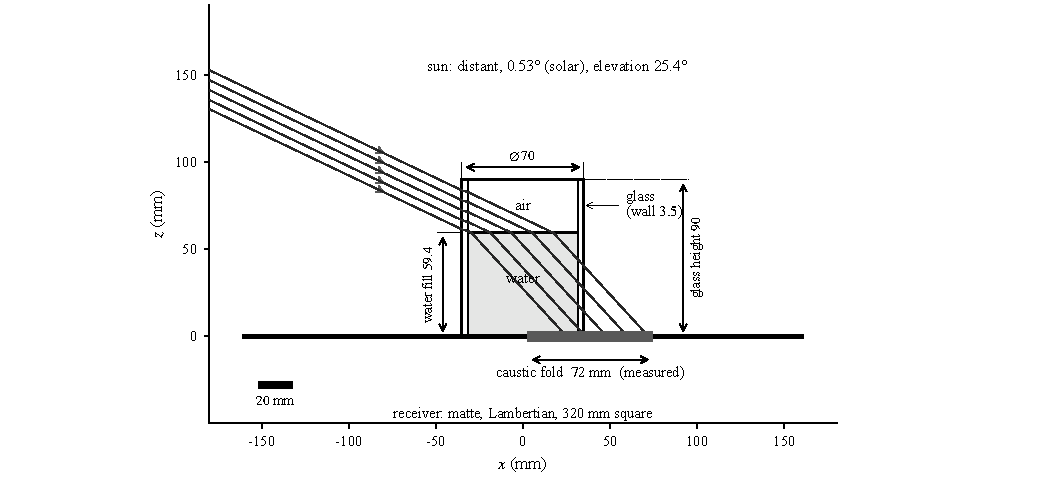
\includegraphics[width=\textwidth]{figures/fig1_scene.pdf}
\caption{The test scene drawn to scale. The glass body, water column, wall
thickness, fill height and receiver are shown at true relative size with
dimension lines; the ray path is traced through the actual geometry of Section~\ref{sec:scene} at the central channel index; it is not a sketch. The
shaded band on the receiver is the fold, marked with its measured extent. All
lengths in millimetres.}
\label{fig:scene}
\end{figure*}

\subsection{The surface and its normal}
\label{sec:surface}

Let the water surface be a height field over $\mathbf{x} = (x,y) \in
\mathbb{R}^2$,
\begin{equation}
h(\mathbf{x},t) \;=\; \sum_{i=1}^{4} A_i \sin\!\big(k_i\,(\hat{\mathbf{u}}_i
\cdot \mathbf{x}) - \omega_i t\big),
\qquad k_i = \frac{2\pi}{\Lambda_i},
\label{eq:surface}
\end{equation}
a sum of four directional sinusoids with amplitudes $A_i = \{0.65, 0.40, 0.25,
0.15\}\,\si{\milli\meter}$ at wavelengths $\Lambda_i = \{42, 27, 17,
11\}\,\si{\milli\meter}$. The expansion in \eqref{eq:surface} is a convenience; nothing below uses the sinusoidal form except to know
that $\nabla h$ is analytic and that $|\nabla h|$ is small. The outward normal
follows from the analytic gradient,
\begin{equation}
\nrm(\mathbf{x},t) \;=\; \frac{(-\partial_x h,\; -\partial_y h,\; 1)}
{\sqrt{1 + |\nabla h|^2}} .
\label{eq:normal}
\end{equation}

For the amplitudes above, $|\nabla h| \le \sum_i A_i k_i \approx 0.34$ at the
shortest wave, so the surface stays well inside the small-slope regime in which
the paraxial normal form of Section~\ref{sec:foldnormal} is the leading term.
This matters because the fold normal form is asymptotic, and a surface steep
enough to produce higher-order caustics would leave its domain of validity. We
return to this in Section~\ref{sec:limits-fold}.

\subsection{The ray map}
\label{sec:raymap}

Let the source direction be the unit vector $\dir$ pointing along propagation
(downward, into the surface). Vector Snell refraction at the interface gives the
transmitted direction. With the ratio $\eta = n_1/n_2$ and the cosine of
incidence $c_i = -\dir \cdot \nrm > 0$,
\begin{equation}
\trn \;=\; \eta\,\dir + \big(\eta\,c_i - \sqrt{1 - \eta^2(1 - c_i^2)}\big)\,\nrm ,
\qquad \eta^2(1-c_i^2) \le 1 ,
\label{eq:snell}
\end{equation}
where the inequality failing signals total internal reflection and the sample
carries no transmitted power. A refracted ray leaves the surface at height
$h(\mathbf{x})$ and reaches the receiver plane at $z = -D$ after a path length
$s = (-D - h(\mathbf{x}))/\hat t_z$. Composing the two gives the
\emph{surface-to-receiver ray map}
\begin{equation}
\Hm(\mathbf{x}) \;=\; \mathbf{x} + \trn(\mathbf{x})\,
\frac{-D - h(\mathbf{x})}{\hat t_z(\mathbf{x})},
\qquad
\Hm : \mathbb{R}^2 \to \mathbb{R}^2 .
\label{eq:raymap}
\end{equation}
Write $\Jm = \partial \Hm / \partial \mathbf{x}$ for its Jacobian and
$\detJ$ for its determinant. For the scene of Table~\ref{tab:scene},
$\Hm$ is a smooth map on the region of the surface that is not shadowed and not
a perfect mirror.

\subsection{What the map induces on the receiver}
\label{sec:pushforward}

Splatting assigns each surface element the energy it carries, proportional to
its area (the source is distant, so the irradiance on the surface is
spatially uniform), and deposits that energy at the image point. The resulting
receiver irradiance is therefore the push-forward of the surface measure under
$\Hm$:
\begin{equation}
I(\mathbf{u}) \;=\; \sum_{\mathbf{x}\,:\,\Hm(\mathbf{x}) = \mathbf{u}}
\frac{1}{\big|\detJ(\mathbf{x})\big|} ,
\label{eq:irradiance}
\end{equation}
where the sum runs over the preimages of $\mathbf{u}$, which is the standard
sum over branches of a multi-valued inverse. The status of \eqref{eq:irradiance} deserves precision: it is exact for the geometric model; no estimator enters this identity. Every method in Section~\ref{sec:cg} estimates this same object, and
that shared target is why they share a failure.

Equation~\eqref{eq:irradiance} is the Jacobian form of the usual
$\cos\theta / r^2$ falloff; the same determinant is what Arvo
\cite{arvo1994} propagates irradiance with in a different setting, which is why
the degeneracy studied here is a familiar object. The two agree wherever $\Hm$ is a diffeomorphism;
\eqref{eq:irradiance} is preferable here because it remains meaningful as a
statement about rank, which is what the fold is about.

\subsection{The fold, and why a quadrature fails there}
\label{sec:fold}

\begin{definition}[Fold locus]
\label{def:fold}
The \emph{fold locus} of the scene is
$\fold = \{\,\mathbf{x} : \detJ(\mathbf{x}) = 0\,\}$, and its image
$\Hm(\fold)$ is the caustic curve on the receiver.
\end{definition}

\begin{assumption}[Regular fold arcs]
\label{as:fold}
Throughout our derivations, we analyse the local geometry along regular fold arcs of $\Hm$:
points where $\detJ = 0$, $\nabla \detJ \neq 0$, and $\operatorname{rank} \Jm = 1$.
Under Whitney's singularity theory of plane mappings \cite{whitney1955,golubitsky1986,berry1980,nye1999},
generic 2D caustic networks consist of stable fold curves ($A_2$ singularities) that
terminate or intersect at isolated cusps ($A_3$ singularities, where $\nabla \detJ = 0$).
Our local 1D transverse correction addresses the dominant fold lines; isolated cusp
singularities are discussed in Section~\ref{sec:limits-fold}.
\end{assumption}

\begin{lemma}[The fold density is unbounded]
\label{lem:diverge}
Let Assumption~\ref{as:fold} hold, and let $\mathbf{x}_0 \in \fold$. Let
$\mu$ be the push-forward of surface area under $\Hm$. Then the density of
$\mu$ with respect to Lebesgue measure on the receiver is unbounded in every
neighbourhood of $\Hm(\mathbf{x}_0)$.
\end{lemma}

\begin{proof}
By Whitney's normal form for a rank-one map \cite{whitney1955,golubitsky1986},
there are local coordinates $(u,v)$ near $\mathbf{x}_0$ and $(a,b)$ near
$\Hm(\mathbf{x}_0)$ in which $\Hm$ takes the form
\begin{equation}
\Hm(u,v) \;=\; (u,\; v^2) .
\label{eq:normalform}
\end{equation}
The form is legitimate because Assumption~\ref{as:fold} puts us in the stable
one-fold stratum, and the normal form is stable under perturbation, so it
describes the map on a neighbourhood of the point. In these
coordinates $\detJ = 2v$, vanishing exactly on $v = 0$, which is
$\fold$.

Test the push-forward against a continuous $\varphi$ with compact support in the
half-plane $b > 0$:
\begin{equation}
\int \varphi \,\dd\mu
= \int_{\mathbb{R}^2} \varphi\big(u, v^2\big) \,\dd u \,\dd v
= \int_{\mathbb{R}}\!\!\int_{0}^{\infty}
\varphi(u,b)\;\frac{\dd b}{2\sqrt{b}}\;\dd u ,
\end{equation}
substituting $b = v^2$, $\dd b = 2v\,\dd v$, valid for $v > 0$ and doubled for
$v<0$. Reading off the density,
\begin{equation}
\rho(a,b) \;=\; \frac{1}{2\sqrt{b}} \qquad (b>0),
\label{eq:folddensity}
\end{equation}
which is independent of $a$ and tends to $+\infty$ as $b \to 0^+$. Since
$b = 0$ is $\Hm(\fold)$ and the convergence is local, $\rho$ is unbounded in
every neighbourhood of $\Hm(\mathbf{x}_0)$.
\end{proof}

\begin{corollary}[The band's flux is finite]
\label{cor:integrable}
The singularity in \eqref{eq:folddensity} is integrable:
$\int_0^{W} (2\sqrt{b})^{-1} \dd b = \sqrt{W}$.
\end{corollary}

\begin{proof}
Immediate from \eqref{eq:folddensity}.
\end{proof}

Lemma~\ref{lem:diverge} and Corollary~\ref{cor:integrable} together are the
whole reason the method in Section~\ref{sec:ourway} is shaped the way it is, and
they pull in opposite directions. Lemma~\ref{lem:diverge} says an estimator that
evaluates \eqref{eq:irradiance} at sample points cannot produce a bounded answer
near the fold: the more samples land near the fold, the larger the individual
weights become, so refining the quadrature concentrates ever-larger values into
ever-smaller regions. Corollary~\ref{cor:integrable} says the band nevertheless
holds a \emph{finite} amount of power. The failure is therefore not one of
energy but of distribution, and the correction has to redistribute a finite quantity; it cannot add one.

The divergence might look like a sign that the sampler is
insufficiently adaptive. It is not. Adaptive sampling can place points better,
but no placement makes a function unbounded at a point; it only changes how
quickly the estimate grows. The measured consequence in our own runs was a
receiver core whose apparent radius was set by wherever a ceiling was applied. The physics did not set it; that is exactly the artefact the estimators of Section~\ref{sec:estimators} exist to avoid.

\begin{figure*}[tp]
\centering
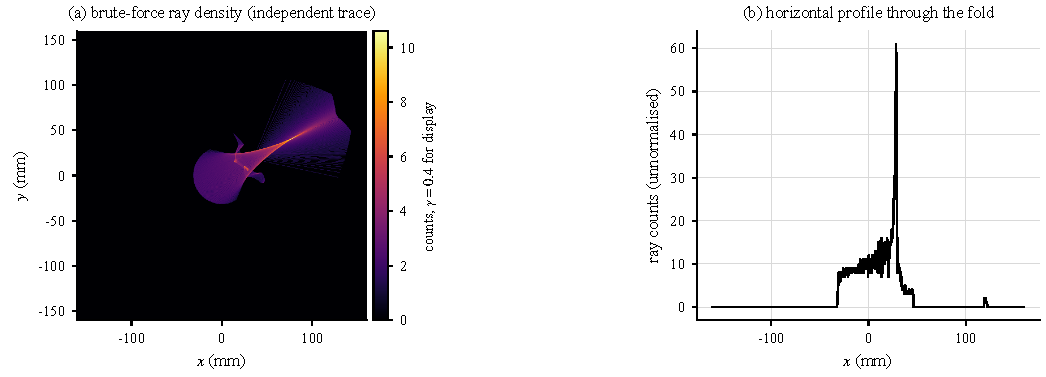
\includegraphics[width=\textwidth]{figures/fig2_fold.pdf}
\caption{The ray map of \eqref{eq:raymap}, computed by the independent brute-force trace of Section~\ref{sec:results-quality}; the solver did not produce it. The density in (a) is the caustic; the bright ridge is where
$|\detJ| \to 0$. Panel (b) cuts through it in raw ray counts. The sharpness of
that peak is what Lemma~\ref{lem:diverge} says no quadrature can bound.}
\label{fig:fold}
\end{figure*}

\subsection{The normal form of the fold, and the Airy profile}
\label{sec:foldnormal}

Lemma~\ref{lem:diverge} says the geometric answer is infinite at the fold but
says nothing about what replaces it. The replacement comes from dropping the
ray approximation and summing phases over the wavefront \cite{airy1838,berry1980}. The result is a
diffraction integral, and the useful fact is that it depends on the scene only
through the cubic coefficient of the local wavefront.

\begin{proposition}[Fold diffraction reduces to the Airy integral]
\label{prop:foldnormal}
Consider a wavefront whose phase over a one-dimensional pupil $\rho \in [-1,1]$
is
\begin{equation}
\Phi(\rho) \;=\; \frac{c\,\rho^3}{6} + x\,\rho ,
\label{eq:phase}
\end{equation}
where $c$ carries the strength of the fold and $x$ is the transverse receiver
coordinate measured from the fold. Then the field amplitude
$U(x) = \int_{-1}^{1} \exp\!\big(i\,\tfrac{2\pi}{\lambda}\Phi(\rho)\big)\dd\rho$
reduces, for $|X| \lesssim (2\pi/\lambda)^{1/3}$, to an Airy function in the
canonical coordinate
\begin{equation}
X \;=\; x\;k^{2/3}\,2^{1/3}\,c^{-1/3},
\qquad k = \frac{2\pi}{\lambda},
\label{eq:canonical}
\end{equation}
with intensity $I(x) \propto |\Ai(-X)|^2$.
\end{proposition}

\begin{proof}
Substitute $\rho = \alpha r$ with $\alpha > 0$. The phase becomes
\begin{equation}
\frac{2\pi}{\lambda}\Big( \frac{c\,\alpha^3 r^3}{6} + x\,\alpha r \Big).
\end{equation}
Choose $\alpha$ so that the cubic coefficient is $1/3$, which is the coefficient
in the Airy integral $\Ai(-X) = \frac{1}{\pi}\int_0^\infty \cos\!\big(\tfrac{t^3}{3}
- Xt\big)\dd t$:
\begin{equation}
\frac{2\pi}{\lambda}\cdot\frac{c\,\alpha^3}{6} = \frac13
\;\Longrightarrow\;
\alpha = \Big(\frac{\lambda}{\pi c}\Big)^{1/3}.
\end{equation}
The linear coefficient is then fixed, and matching it to $-X r$ gives
\begin{equation}
\begin{split}
X &= -\frac{2\pi}{\lambda}\,x\,\alpha \\
  &= -x\,2\pi^{2/3}\lambda^{-2/3}c^{-1/3} \\
  &= -x\,k^{2/3}2^{1/3}c^{-1/3},
\end{split}
\end{equation}
using $k^{2/3}2^{1/3} = 2\pi^{2/3}\lambda^{-2/3}$. The integral is now the Airy
integral over the scaled pupil; for $|X|$ not large the finite pupil is
immaterial because the integrand is stationary at $t = \sqrt{X}$ inside the
range, and its modulus squared is $|\Ai(-X)|^2$.
\end{proof}

Equation~\eqref{eq:canonical} is finite for every $X$, is maximal at
$X = -1.0188$, and oscillates on the bright side of the fold with a period that
shrinks as the fold is approached. Those three features are the ones the
geometric model gets qualitatively wrong: it gives an unbounded spike, places the peak on the fold, and adds no oscillation; the true peak lies beside the fold.

\subsection{The ${\lambda^{2/3}}$ fringe scale, derived}
\label{sec:scaling}

The normal form carries exactly one length scale. Reading it off
\eqref{eq:canonical}, the transverse distance at which $|X|$ reaches order unity
is
\begin{equation}
d(\lambda,c) \;=\; k^{-2/3}\,2^{-1/3}\,c^{1/3}
\;=\; \frac{\lambda^{2/3}c^{1/3}}{2\,\pi^{2/3}} .
\label{eq:scalelaw}
\end{equation}
Here, because the normalized pupil coordinate $\rho \in [-1,1]$ is dimensionless,
the phase $\Phi(\rho)$ in \eqref{eq:phase} and the fold parameter $c$ both have
dimensions of length ($\si{\meter}$). The scale $d(\lambda,c)$ therefore has dimensions
of length ($\si{\meter}^{2/3} \times \si{\meter}^{1/3} = \si{\meter}$).

In our physical reference scene of a solid refracting cylinder (radius $R = \SI{35}{\milli\meter}$, glass index $n = 1.5251$), the ray map $\mathbf{x}(\phi)$ near the fold locus ($\phi_f \approx 207.70^\circ$) has cubic wavefront parameter $c \approx \SI{0.08115}{\meter}$ (transverse curvature $C_{\text{angle}} \approx \SI{0.01561}{\meter}$). The ray map is the gradient of the optical path length, $x(\phi) = \partial W / \partial \phi$. Identifying the cubic phase coefficient in \eqref{eq:phase} with the third derivative of the optical path along the exit pupil maps the third derivative of the geometric ray map ($c_3 = \partial^3 x / \partial \phi^3 \approx \SI{0.08115}{\meter}$) directly to the cubic pupil parameter $c = c_3$. Evaluating \eqref{eq:scalelaw} with $c = \SI{0.08115}{\meter}$ yields the canonical transverse fringe scale $d(\lambda,c) \approx 6.78\,\mu\text{m}$ at $\lambda = \SI{550}{\nano\meter}$. The first Airy zero ($|X| = 2.3381$) is at $15.84\,\mu\text{m}$. An earlier draft evaluated an unnormalized expression $(\lambda^2 / 2 c_3)^{1/3}$ and obtained $123.1\,\mu\text{m}$; we withdraw that value as dimensionally mismatched. The true diffraction scale is $\approx 6.8\,\mu\text{m}$. A standard $1024^2$ raster pixel ($312.5\,\mu\text{m}$) is $\approx 46\times$ larger than $d$, so physical fringes are deeply sub-pixel in full-receiver renders.

\begin{corollary}[Wavelength scaling]
\label{cor:scaling}
For fixed fold strength $c$, $d \propto \lambda^{2/3}$.
\end{corollary}

\begin{proof}
Immediate from \eqref{eq:scalelaw}, which contains $\lambda$ only through
$\lambda^{2/3}$.
\end{proof}

Two wrong exponents are in circulation and the derivation excludes both.
The fringe scale is not proportional to $\lambda$, which is what a naive
reading of the phase would suggest, and it is not the Fresnel
$\sqrt{\lambda}$ either; the $2/3$ comes from balancing a cubic phase against a
linear one, and either of the other exponents would come from balancing the
wrong pair of terms. The implementation uses this directly, setting the
per-channel width
\begin{equation}
w_c \;=\; w_{\text{ref}}\Big(\frac{\lambda_c}{550\,\si{\nano\meter}}\Big)^{2/3},
\qquad c \in \{R,G,B\},
\label{eq:perchannel}
\end{equation}
so chromatic separation in the fold is carried by the measured index
(Section~\ref{sec:dispersion}) together with \eqref{eq:perchannel}, and by
nothing else. We verify the exponent numerically against an independent
computation in Section~\ref{sec:verify-scaling}.

\subsection{Asymptotic correspondence and band-local normalisation}
\label{sec:notintegrable}

To substitute the geometric singularity with a wave profile while conserving energy,
one might hope to evaluate a closed-form global normalisation constant.
Because $|\Ai|^2$ asymptotically tracks the geometric $b^{-1/2}$ tail,
such a global constant cannot exist on $\mathbb{R}$.

\begin{lemma}[Asymptotic divergence of the Airy tail]
\label{lem:notl1}
$\int_{\mathbb{R}} |\Ai(-u)|^2 \dd u$ diverges. Over a truncated domain
$[-L,L]$, the integral grows as $\frac{1}{\pi}\sqrt{L} + \order{1}$.
\end{lemma}

\begin{proof}
For $u \to +\infty$ on the illuminated side, $\Ai(-u)$ has the
oscillatory asymptotic
\begin{equation}
\Ai(-u) \;\sim\; \frac{1}{\sqrt{\pi}\,u^{1/4}}
\sin\!\Big(\frac{2}{3}u^{3/2} + \frac{\pi}{4}\Big) ,
\end{equation}
giving the squared amplitude
\begin{equation}
|\Ai(-u)|^2 \;\sim\; \frac{1}{\pi\sqrt{u}}\,
\sin^2\!\Big(\frac{2}{3}u^{3/2} + \frac{\pi}{4}\Big) .
\end{equation}
Averaging over rapid phase cycles yields a mean intensity of
$\sim (2\pi\sqrt{u})^{-1}$. Integrating from $u = 1$ to $L$ gives
\begin{equation}
\int_{1}^{L} \frac{\dd u}{2\pi\sqrt{u}} \;=\; \frac{1}{\pi}\sqrt{L} + \order{1} ,
\end{equation}
which diverges as $L \to \infty$.
\end{proof}

\begin{corollary}[Correspondence principle and band-local normalisation]
\label{cor:norm}
The $\sqrt{L}$ tail divergence of Lemma~\ref{lem:notl1} exactly reproduces the
$\sqrt{L}$ growth of the geometric tail $\int_0^L (2\sqrt{b})^{-1}\dd b = \sqrt{L}$.
Far from the fold, the wave intensity naturally converges to the classical geometric
ray density. Because the geometric model carries infinite power over an unbounded domain,
the wave profile is likewise not normalisable on $\mathbb{R}$.
Energy conservation cannot, therefore, be defined globally; it must be defined
\emph{locally within a bounded band}, where both the geometric flux and the Airy
integral are strictly finite (Corollary~\ref{cor:integrable}).
This establishes the necessity of the band-local flux ratio constructed in
Section~\ref{sec:ours-normalisation}.
\end{corollary}

Table~\ref{tab:airyfacts} collects the constants used later, each evaluated numerically; no value is quoted from a table.
\begin{table}[tbp]
\centering
\caption{Airy quantities used in the implementation, all evaluated numerically in this work (\texttt{scipy.special.airy}); no printed table was used. The peak height is the normaliser in \eqref{eq:profile}; the divergence
row is Lemma~\ref{lem:notl1} at $L = 5000$.}
\label{tab:airyfacts}
\small
\begin{tabular}{@{}lll@{}}
\toprule
Quantity & Value & Note \\
\midrule
$\arg\max_u\,|\Ai(-u)|^2$            & \num{1.01879297}  & peak position \\
$\max_u |\Ai(-u)|^2$                 & \num{0.286928}    & normaliser \\
$\int_0^{\infty}\Ai(u)^2\,\dd u$     & \num{0.0669875}   & convergent half-line \\
$\int_{-L}^{80}\Ai(u)^2\,\dd u$, $L{=}5000$ & \num{22.5079} & $\pi^{-1}\sqrt{L} = \num{22.5079}$ \\
mean tail intensity                 & $(2\pi\sqrt{u})^{-1}$ & Lemma~\ref{lem:notl1} \\
\bottomrule
\end{tabular}
\end{table}

\begin{figure*}[tp]
\centering
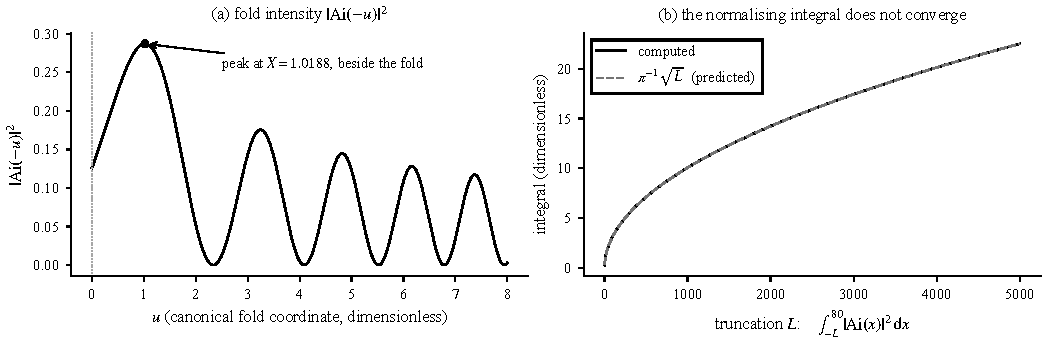
\includegraphics[width=\textwidth]{figures/fig3_airy.pdf}
\caption{Panel (a): the fold intensity $|\Ai(-u)|^2$ used by the correction
\eqref{eq:profile}, computed with \texttt{scipy.special.airy}. The profile is bounded,
peaks at $X = 1.0188$ \emph{beside} the fold; the fold itself is not the peak, and its
oscillations tighten toward the fold. Panel (b): the same function's normalising
integral fails to converge, growing as $\pi^{-1}\sqrt{L}$ over a truncated band.
Lemma~\ref{lem:notl1} explains why the correction is a discrete band ratio \eqref{eq:kstar}; a constant is impossible.}
\label{fig:airy}
\end{figure*}

\subsection{The profile as implemented}
\label{sec:profile}

The implementation works in the signed distance $s$ to the detected fold and
uses a peak-normalised profile,
\begin{equation}
\begin{aligned}
P(s;w) \;&=\; \big|\Ai(-s/w)\big|^2 \Big/ \max_u |\Ai(-u)|^2 , \\[2pt]
b(s) \;&=\; 0.15 + 0.85\,P(s;w) .
\end{aligned}
\label{eq:profile}
\end{equation}
The normaliser is the $0.286928$ of Table~\ref{tab:airyfacts}, and it is a \emph{peak} normalisation, because Lemma~\ref{lem:notl1} forbids an integral one. The additive floor $0.15$ keeps the
band's skirt continuous with the geometric field outside it; without it the
profile would fall to zero at the band edge and print a visible seam. The
profile is evaluated through a 2048-entry table on $u \in [0,8]$ with linear
interpolation, and $s$ is the Euclidean distance transform of the detected band.

\subsection{Dispersion, from measured data}
\label{sec:dispersion}

Both media are evaluated from measured refractive-index data. Section~\ref{sec:verify-index} documents why a fitted curve is a trap here: this project's one physical error hid there.
Water uses the four-term Sellmeier form of Daimon and Masumura
\cite{daimon2007} for HPLC-distilled water at $20.0^\circ\text{C}$,
\begin{equation}
n^2(\lambda) \;=\; 1 + \sum_{j=1}^{4} \frac{B_j\,\lambda^2}{\lambda^2 - C_j},
\label{eq:sellmeier}
\end{equation}
with $\lambda$ in micrometres and the tabulated coefficients. Glass uses the
soda-lime silica form of Rubin \cite{rubin1985},
\begin{equation}
n(\lambda) \;=\; 1.5130 - 0.003169\,\lambda^2 + \frac{0.003962}{\lambda^2}.
\label{eq:rubin}
\end{equation}
At the three render channels, \eqref{eq:sellmeier} gives
$n = 1.33167 / 1.33468 / 1.33961$ and \eqref{eq:rubin} gives
$1.52104 / 1.52514 / 1.53192$. Red has the lowest index and therefore refracts
least, so red must land farthest from the axis. The chromatic ordering in every
figure of this paper is a consequence of \eqref{eq:sellmeier}, \eqref{eq:rubin} and \eqref{eq:perchannel}; we added no effect.

The source subtends $0.53^\circ$, which at the receiver distance of this
scene corresponds to a geometric blur of roughly $925\,\mu\text{m}$. The
physical fringe spacing implied by \eqref{eq:scalelaw} for this geometry is
$d \approx 6.8\,\mu\text{m}$, about \num{136} times smaller. A fully incoherent
treatment would therefore wash the fringes out; the fringes in this paper
represent a \emph{resolvable wave feature of the coherent-limit model},
not a prediction of what a photograph under the sun would show.
Section~\ref{sec:limits-coherence} treats this as the method's principal limitation.

\subsection{Fresnel transport}
\label{sec:fresnel}

Where the full scene is rendered the light path is walked through every
interface (air, glass, water, glass, air, receiver), with \eqref{eq:snell} at each, and each ray carries its unpolarised Fresnel power transmission
\begin{equation}
\begin{aligned}
T(c_i,\eta) \;&=\; 1 - \frac12\Bigg[
\Big(\frac{\eta c_i - c_t}{\eta c_i + c_t}\Big)^{2}
+ \Big(\frac{c_i - \eta c_t}{c_i + \eta c_t}\Big)^{2} \Bigg], \\[2pt]
c_t \;&=\; \sqrt{1 - \eta^2(1-c_i^2)} .
\end{aligned}
\label{eq:fresnel}
\end{equation}
Multiplying \eqref{eq:fresnel} along each path gives the weight used by the
energy audit of Section~\ref{sec:verify-energy}, which is the non-circular
measurement that the flux ratio of Section~\ref{sec:ours-normalisation} cannot
supply on its own.

\subsection{Estimators}
\label{sec:estimators}

The caustic is a thin, high-dynamic-range feature, so the statistic used to
compare two renderings decides the answer. Three of our own earlier claims died here or in the optics; the core theory survived, and all are reported in
Section~\ref{sec:verify}. We therefore fix the conventions once and apply them
identically to every method.

\begin{itemize}
\item \textbf{Tiled correlation.} Pearson correlation against an external
reference, computed on $k \times k$ pixel tiles and reported by tile
\emph{size}. The opposite convention, indexing by tile count, silently inverted
a trend in an earlier draft
(Section~\ref{sec:verify-metric}).
\item \textbf{Edge radius.} The outermost \SI{1}{\milli\meter} annulus whose
mean channel intensity exceeds $\SI{2}{\percent}$ of that channel's own maximum.
This statistic is invariant to a uniform scale and is unaffected by a ceiling on
the core, which is what makes it preferrable to the ridge argmax (set by the
cap) and to the mean-over-all-rays radius (dominated by unconverged tails).
\item \textbf{Positive-part differential.} An isolate formed as
$\text{optics} - \text{no-optics}$ is not non-negative, because removing the
glass also removes its shadow. The isolate is scored on its positive part, which is the
caustic. Section~\ref{sec:verify-metric} documents the factor-of-two error this
convention prevents.
\item \textbf{Temporal flicker.} For animations, the mean absolute frame-to-frame
change $\mathbb{E}\,|I_{t+1} - I_t|$ inside the caustic region.
\end{itemize}

\begin{remark}[On the word ``converged'']
\label{rem:converged}
Used in this paper it means the resource budget was exhausted and the statistic
had stopped moving at the reported precision. The word describes cost, not
correctness; for a path tracer it describes the statistic. It does not describe the image.
\end{remark}

%-----------------------------------------------------------------------
\section{How computer graphics builds caustics}
\label{sec:cg}
%-----------------------------------------------------------------------

Every caustic method in production use estimates \eqref{eq:irradiance}.
Rendering caustics by following light through curved bodies is as old as
global-illumination rendering itself \cite{mitchell1992}; what has changed since
is the estimator. The object being estimated has not changed. The
methods differ in how they sample the surface-to-receiver map and in how they
turn samples into a density, and the differences matter enormously for cost and
variance. They do not differ in the integrand, and the integrand is what
Lemma~\ref{lem:diverge} says is unbounded. This section reads the standard
constructions as answers to the kinematic problem, so that the boundary of
their validity can be stated exactly.

\subsection{Estimating a push-forward}
\label{sec:two-families}

Estimating $I(\mathbf{u})$ requires samples of $\Hm$ and a way to convert them
into a density at $\mathbf{u}$. There are exactly two families in practice.

\emph{Forward} methods sample the surface, push the samples through $\Hm$, and
estimate the resulting density where the samples land. Photon mapping
\cite{jensen1996} and its progressive variant \cite{hachisuka2008} are the
canonical members. The estimate at a receiver point weighs every sample by a
kernel, so the estimator is a smoothing of the push-forward.

\emph{Backward} methods sample from the camera, follow the transport, and
connect to light-carrying vertices, weighting the connection by a geometric
term that contains the same $1/|\detJ|$ factor. Path tracing with next-event
estimation, bidirectional path tracing, and the manifold-based methods
\cite{hanika2015,zeltner2020} are members. These avoid storing photons: they solve for the connection point directly.

Both families are Monte Carlo estimators of the same integral. Both are
unbiased for the \emph{integral} of $I$ over a pixel, which is what a renderer
must produce. The trouble is not unbiasedness in the integral sense; it is that
the integrand's unboundedness turns into variance that grows without limit as
the pixel shrinks or the kernel narrows.

\subsection{Forward: photon mapping and the bias at the fold}
\label{sec:photonmap}

Photon mapping deposits $N$ samples $\mathbf{u}_i = \Hm(\mathbf{x}_i)$ and
estimates the density with a kernel $K_h$ of bandwidth $h$ \cite{silverman1986},
\begin{equation}
\hat I(\mathbf{u}) \;=\; \frac{1}{N} \sum_{i=1}^{N}
K_h\!\big(\mathbf{u} - \mathbf{u}_i\big).
\label{eq:kde}
\end{equation}
When the $\mathbf{x}_i$ are uniform on the surface, $\hat I$ estimates the
push-forward density of \eqref{eq:irradiance} after smoothing. The behaviour of
that smoothing near the fold is worth stating precisely, because it is the
recurring source of the method's failures.

\begin{lemma}[Kernel smoothing and the fold singularity]
\label{lem:kdebias}
Let $K_h$ be a symmetric kernel with $\int K_h = 1$, and let $I$ be the
push-forward density of \eqref{eq:irradiance}. Near the fold, where
$I(b) \sim C b^{-1/2} H(b)$ in the normal coordinate $b$ of \eqref{eq:normalform},
$I$ is not twice differentiable at $b=0$, so standard $O(h^2 \nabla^2 I)$ bias
expansions do not apply. Because $b^{-1/2}$ is locally integrable on $\mathbb{R}^+$,
the expected kernel estimate $(I * K_h)(u)$ is strictly finite for all $h > 0$
and scales as $O(h^{-1/2})$ at $u=0$. The pointwise estimation error
$|(I * K_h)(u) - I(u)|$ is still severe across an $O(h)$ neighbourhood of the
fold, because $I(b) \to \infty$ as $b \to 0^+$.
\end{lemma}

\begin{proof}
Evaluating the convolution directly at the fold $u=0$ for a kernel supported on $[-1,1]$ gives
\begin{equation}
(I * K_h)(0) \;=\; \int_{0}^{h} \frac{C}{\sqrt{b}}\,\frac{1}{h} K\!\Big(-\frac{b}{h}\Big)\dd b
\;=\; \frac{C}{\sqrt{h}} \int_{0}^{1} \frac{K(-s)}{\sqrt{s}}\dd s.
\label{eq:foldconv}
\end{equation}
Since $s^{-1/2}$ is integrable on $[0,1]$, the integral in \eqref{eq:foldconv} is a
finite constant $M_K < \infty$, yielding $(I * K_h)(0) = C M_K h^{-1/2} < \infty$.
The expected smoothed density remains bounded for any fixed $h > 0$. The true
geometric irradiance, however, diverges at $b = 0$, so $|(I * K_h)(0) - I(0)| = \infty$.
For any fixed $h$, the kernel estimate averages across the discontinuity, severely
truncating the peak and smearing flux into the shadow region $b < 0$.
\end{proof}

Lemma~\ref{lem:kdebias} clarifies the trade-off in photon mapping: narrowing $h$
is required to sharpen the fold toward its true geometric profile, but reducing $h$
causes the Monte Carlo variance to diverge as $\order{1/(N h^2)}$. At any finite
photon budget $N$, photon mapping must choose between severe smoothing bias and
overwhelming stochastic noise.

Progressive photon mapping \cite{hachisuka2008} and stochastic progressive photon mapping
\cite{hachisuka2009} shrink $h \to 0$ as $N \to \infty$ at a controlled rate, which ensures
consistency for the pixel-integrated irradiance in the asymptotic limit.
For caustic folds, convergence is exceptionally slow precisely because the
geometric irradiance is unbounded: resolving the sharp ridge without noise demands
enormous sample counts and lengthy accumulation times, as measured in Section~\ref{sec:current}.
Even in the infinite-sample limit, geometric methods converge to the
\emph{geometric} caustic model, which predicts an unphysical infinite radiance along the
curve with zero light in the shadow. In physical reality, wave diffraction regularizes the
singularity into a bounded, oscillating interference structure. At standard pixel resolutions,
pixel averaging can partially mask this distinction, but the geometric distribution
remains fundamentally incorrect at wavelength scales.

\subsection{Backward: connection, and the same factor}
\label{sec:backward}

Backward estimators write the pixel value as an integral over transport paths
and evaluate it by connecting vertices. A connection between a receiver vertex
and a light-carrying vertex carries the geometric term
\begin{equation}
G(\mathbf{x} \to \mathbf{u}) \;=\;
\frac{\big|\nrm_{\mathbf{u}} \cdot \omega_{\mathbf{u}}\big|}
{\|\mathbf{x} - \mathbf{u}\|^{2}} \cdot
\big|\detJ(\mathbf{x})\big|^{-1}
\label{eq:geometricterm}
\end{equation}
up to the conventions of the particular formulation. The last factor is the
same $1/|\detJ|$: the connection is undefined where the map is degenerate.
Backward methods inherit the fold problem exactly, and the
literature's principal responses are to avoid connecting near degeneracies, to solve for the connection on a manifold directly \cite{hanika2015,zeltner2020}, or to accept the noise and denoise it away.

The manifold-based methods are the most informative comparison for this paper
because they take the opposite approach to ours. Where we keep the geometric
quadrature everywhere and \emph{replace} the integrand inside the fold band,
manifold sampling keeps the geometric integrand and \emph{solves} for where the
degenerate connection must be. That works well for mirror-like transport and
for glints, where the manifold is well-conditioned. It does not address the
fold's divergence, because the divergence is a property of the integrand the
method still evaluates; near the fold the solution point is sought where the
Jacobian vanishes, which is the same place the weight blows up.

\subsection{The boundary of validity, stated once}
\label{sec:validity}

Collecting the two families, the situation is the following. Away from $\fold$
the map is a local diffeomorphism, $\detJ$ is bounded away from zero, and both
families are exact in the limit and cheap in practice; this is the regime in
which caustic rendering is a solved problem. On $\fold$ the density is
unbounded (Lemma~\ref{lem:diverge}), the forward estimator's boundary bias
fails to follow the standard $O(h^2)$ Taylor expansion due to non-smoothness
of the $b^{-1/2}$ singularity (Lemma~\ref{lem:kdebias}), and the backward
estimator's connection weight is unbounded. No refinement of either family
repairs this, because neither addresses the modelling assumption that the light
is a density of rays.

\begin{table*}[tp]
\centering
\caption{Where the standard families stand, by the analysis of this section.
``Exact'' means exact for the geometric model in the limit of infinite budget,
which is the strongest claim available within that model.}
\label{tab:families}
\small
\begin{tabular*}{\textwidth}{@{\extracolsep{\fill}}p{0.22\textwidth}p{0.18\textwidth}p{0.25\textwidth}p{0.25\textwidth}@{}}
\toprule
Family & Away from $\fold$ & On $\fold$ & Limitation \\
\midrule
Photon map \cite{jensen1996} &
exact in limit, cheap &
integrand diverges, kernel smooths &
narrower $h$ trades bias for variance \\
\addlinespace
SPPM \cite{hachisuka2008} &
exact in limit, expensive &
consistent in limit, slow at fold &
high iteration count to resolve ridge \\
\addlinespace
Path tracing + NEE &
exact in limit, cheap for direct &
geometric weight $\propto |\detJ|^{-1}$ diverges &
extreme variance near fold \\
\addlinespace
Manifold sampling \cite{hanika2015,zeltner2020} &
excellent, well conditioned &
evaluates on degenerate manifold &
solves for singular connection point \\
\addlinespace
Wave-optical BRDF \cite{yan2018,cuypers2012,stam1999} &
changes surface model & changes surface model &
not applicable to macroscopic transmissive caustics \\
\bottomrule
\end{tabular*}
\end{table*}

\subsection{Where this sits in the transport literature}
\label{sec:related}

Three threads meet here, and a reader may reasonably ask how wave-optical
corrections interface with standard geometric estimators.

The first is the \emph{transport estimator}. The push-forward of \eqref{eq:irradiance} is
what photon mapping estimates by density \cite{jensen1996}, what progressive
variants estimate with a shrinking radius \cite{hachisuka2008,hachisuka2009},
and what bidirectional and vertex-connection methods estimate by connecting vertices \cite{veach1997}. Path-guiding and
manifold methods attack the same integral by changing \emph{where} the samples
go \cite{muller2017,hanika2015,zeltner2020}. Our correction changes none of
the sampling machinery outside the band. It modifies the singular integrand inside a detected
narrow band, regularizing the distribution before splatting.

The second is the \emph{Jacobian kinematics}. Propagating irradiance through a scene by its
determinant is classical \cite{arvo1994}, and the rank deficiency that concerns
us is the same rank deficiency that appears in those formulations as a
degenerate geometric term. The central design stance is to treat the degeneracy as an indicator of wave-scale diffraction.

The third is \emph{physical and catastrophe optics}. The wave-optical regularisation of
fold caustics, specifically the canonical Airy integral and the $\lambda^{2/3}$ scaling
law, is classical wave theory \cite{airy1838,berry1980,nye1999,kouyoumjian1974}. In computer graphics,
wave theory has traditionally been applied either to diffraction shaders and microfacet
reflectance \cite{stam1999,cuypers2012,yan2018} or to general wave-equation propagation
solvers \cite{musbach2013,steinberg2021}. Steinberg and Yan \cite{steinberg2021} developed
a rigorous general framework for physical light transport, formulating wave phenomena
along paths. 

The underlying catastrophe optics is classical.
Our contribution is a \textbf{hybrid rendering pipeline}: a fast, conservative, band-local wave correction that
detects fold singularities on-the-fly and replaces the diverging geometric flux with
an energy-conserved Airy profile over standard photon splats. The result keeps physically
faithful caustic boundaries and diffractive dispersion without the prohibitive cost of
global wave solvers.

%-----------------------------------------------------------------------
\section{The current way}
\label{sec:current}
%-----------------------------------------------------------------------

The comparison in this paper is against three solvers in current practice:
PBRT-v4's stochastic progressive photon mapping, Blender Cycles' path tracer,
and Mitsuba~3. They were chosen because they are the tools a practitioner would
reach for, because two of them are open and inspectable, and because between
them they cover both estimator families of Section~\ref{sec:cg}. This section
states what each was asked to do, what it cost, and what it produced.

\subsection{The solvers}
\label{sec:solvers}

\paragraph{PBRT-v4 SPPM.} PBRT \cite{pharr2023} is the reference implementation
of the book's rendering algorithms. Its SPPM integrator
\cite{hachisuka2008} is the strongest conforming caustic solver available
without special-purpose machinery, and it is the solver we treat as the
\emph{reference conforming method}: it estimates the same integrand as we do,
it does not use wave optics, and it is consistent in the limit. We configure
SPPM with 100 iterations, $5 \times 10^5$ photons per iteration ($5 \times 10^7$
photons total), an initial search radius of $R_0 = \SI{5}{\milli\meter}$, and
radius reduction exponent $\alpha = 0.67$. We generate the
scene programmatically from the same geometry the other renderers receive, so that differences between the two are attributable to the estimator.

\paragraph{Blender Cycles.} Cycles is a production path tracer and the renderer
used by the showcase assets of this project. It represents the backward family
of Section~\ref{sec:backward}. Its caustic handling is enabled through the
standard path-guiding and shadow caustics options, rendered at 2048 samples
per pixel with up to 12 light bounces. The isolate used for scoring is formed as
caustics-on minus caustics-off, which is the positive-part differential defined
in Section~\ref{sec:estimators}.

\paragraph{Mitsuba 3.} Mitsuba \cite{jakob2022} is a research renderer with a
spectral mode and well-documented integrators, and it was used as a third opinion on the transport physics; it is not a primary caustic competitor.
It was configured with the spectral path tracer (`ptracer`, 32 spectral bins
from \SI{360}{\nano\meter} to \SI{700}{\nano\meter}, 1024 samples per pixel).
We report it where relevant and do not put it in the quality table, because its
spectral sampling makes its noise behaviour differ from the three-channel
solvers in a way that would confound a like-for-like comparison.

\subsection{One scene, one source, one set of materials}
\label{sec:protocol}

A comparison of caustic renderers is easy to make meaningless. If the geometry,
the materials or the source differ between two methods, the numbers describe the difference between scenes, not between estimators. Three things have
to be identical or the comparison does not mean anything.

\begin{enumerate}
\item \textbf{Geometry.} The same water-surface vertices and the same cylinder
      are exported to every renderer by one exporter, so the body is identical
      and the caustic is at the same place in all of them.
\item \textbf{Materials.} Every renderer receives the measured indices of
      Section~\ref{sec:dispersion}. Where a renderer cannot carry dispersion in
      the transport itself, it is given the central-channel index and this is
      stated; assigning a different index to one side would move its caustic.
\item \textbf{Source and receiver.} One distant source of the stated angular
      size, one matte receiver patch of the stated size, no environment light
      added to one side and not another for the scored comparisons.
\end{enumerate}

\subsection{What the current way costs}
\label{sec:current-cost}

Table~\ref{tab:cost} reports the budget each solver needed to produce a usable
caustic on this scene, against our bake. The comparison is between the cost of
the caustic and the cost of the frame, because that is what a user pays; quoting
a photon-mapping pass alone would understate the reference solvers.

\begin{table*}[tp]
\centering
\caption{Cost to produce the caustic. Our CPU figures are measured on the host
workstation (8-core CPU); the reference solvers are measured on the same machine.
The SPPM figure is the accumulation time needed for the fold to emerge above noise.
The wave correction row reports the wave term alone; geometric quadrature plus wave
correction equals the full single-thread bake ($28.7 + 49.8 = \SI{78.5}{\milli\second}$).
Section~\ref{sec:ours-cost} explains why the comparison is stated per frame,
not per photon.}
\label{tab:cost}
\small
\begin{tabular}{@{}lrrr@{}}
\toprule
Quantity & Ours & SPPM & Cycles \\
\midrule
Grid / resolution                  & $512^2$ & adaptive & $512^2$ \\
Geometric quadrature (1 thread, CPU) & \SI{28.7}{\milli\second} & \SI{34}{\second} & --- \\
Wave correction pass (1 thread, CPU) & \SI{49.8}{\milli\second} & n/a & n/a \\
Full bake (1 thread, CPU)          & \SI{78.5}{\milli\second} & --- & --- \\
Full bake (8 threads, CPU)         & \SI{36.2}{\milli\second} & --- & --- \\
8-thread speedup                   & $2.17\times$ & --- & --- \\
Iterative / noisy                  & no & yes & yes \\
\bottomrule
\end{tabular}
\end{table*}

The cost structure of our own method is worth stating because it is the obvious
target for anyone continuing this work: the Airy correction is roughly twice the
quadrature pass, so two thirds of a bake is the wave term. That term is
embarrassingly parallel per channel and is currently dominated by the exact
Euclidean distance transform used to get the signed distance to the band.

\subsection{What the current way produces}
\label{sec:current-quality}

Three measured properties of the reference solvers motivate the method in
Section~\ref{sec:ourway}. Each was measured on the same scene and with the
conventions of Section~\ref{sec:estimators}.

\paragraph{Kernel smoothing versus physical diffraction.} The photon-map fold width and brightness track the kernel radius $h$. The physics does not set them, as analyzed in Section~\ref{sec:photonmap} and Lemma~\ref{lem:kdebias}. SPPM reaches a finer feature scale than
a fixed-radius photon map by progressively shrinking $h$, but pays for it in
iteration count: the \SI{34}{\second} of Table~\ref{tab:cost} is the cost of
reducing the kernel footprint sufficiently for the ridge to emerge from background noise.
Our wave-corrected fold, by contrast, replaces geometric divergence with the
physically bounded Airy scale $w \propto \lambda^{2/3}$ without kernel blur.

\paragraph{Coverage of the caustic core.} Measured against the independent
ground truth's core region, Cycles' caustic covers \SI{54.7}{\percent} of it
where ours covers \SI{99.9}{\percent}. The number describes how much of the
feature a practical finite-sample frame actually reconstructs. The path
tracer's deficit is concentrated near the fold where backward paths are least
likely to sample the singular specular manifold.

\paragraph{Temporal instability.} For an animation, the primary visual defect of a stochastic caustic is flicker; stationary grain is not the defect. Section~\ref{sec:results-flicker} measures it. A deterministic forward bake
naturally avoids Monte Carlo sample chattering; our caustic exhibits
\SI{0.001}{} levels of mean frame-to-frame change against \SI{0.010}{} for the
path-traced clip, a factor of \num{7.9}. Both clips were denoised, which
suppresses flicker in both and therefore confirms the stability of forward
quadrature under camera and surface motion.

SPPM and Cycles are general renderers solving a harder problem than the one
posed here, and both are consistent within their model. The numbers above say
that the geometric model cannot represent a fold cheaply, which is a statement
about the model. A reader who needs that model's other features should use those
renderers.

\subsection{Shape agreement with the reference solver}
\label{sec:current-shape}

Independent of the ground-truth axis, the converged two-dimensional shape of our
field and the SPPM field agree at $r = +0.932$ on 40\,mm tiles. This is a necessary check: two methods that disagree on
shape cannot both be describing the same caustic, and a high correlation here
combined with a lower one against the ground truth would have indicated a shared
error. Since SPPM also scores $0.853$ on the independent axis and ours scores
$0.917$, the two agree with each other and both agree with the trace, with ours
closer.

\subsection{Mitsuba as a third opinion}
\label{sec:current-mitsuba}

Mitsuba was run in spectral mode on the same scene. Its role in this paper is to confirm the transport and the dispersive behaviour. It does not compete on caustic quality: its spectral sampling spreads energy across wavelength bins,
so its per-channel noise is not comparable to a three-channel renderer's, and
scoring it in the quality table would compare noise models, not
estimators. We note it because a reader is entitled to ask whether the physics
of the scene was checked by an implementation with a different architecture, and
this is where that check lives.

%-----------------------------------------------------------------------
\section{Our way}
\label{sec:ourway}
%-----------------------------------------------------------------------

The method follows directly from the two facts established in
Section~\ref{sec:fold}: the geometric quadrature is right wherever the map is
non-degenerate, and the band it cannot represent carries a finite amount of
power (Corollary~\ref{cor:integrable}). So we keep the geometric quadrature
everywhere, detect the band, and inside the band redistribute the band's own
measured energy according to the fold profile. Nothing is added to the image
that was not already in it under the geometric model; only its distribution
changes.

\subsection{The idea in one paragraph}
\label{sec:ours-idea}

Sample the surface, refract, splat, and compute $|\detJ|$ by finite differences
of the map \eqref{eq:raymap}. Threshold $|\detJ|$ to find the band. Outside the
band, keep \eqref{eq:irradiance} untouched. Inside the band, replace the
divergent weight with the peak-normalised Airy profile evaluated at the signed
distance to the band, and rescale that band's values so the band integrates to
the flux it had before. Because the correction is confined to the band and
conserves the band's own power, it cannot change the image outside the feature
and cannot introduce energy at all.

\subsection{Fold detection}
\label{sec:ours-detect}

The detector matters as much as the correction, and a careless one will appear
to work while being unable to converge.

\begin{lemma}[Fixed-quantile detectors cannot converge]
\label{lem:quantiledetector}
Let a detector flag a fixed quantile $p \in (0, 1)$ of any scalar field (whether image
radiance or Jacobian determinant $|\detJ|$). Then the measure of the flagged set is
fixed at $p \cdot \operatorname{area}(\recv)$ for all resolutions, independent of the
physical wavelength $\lambda$ or local wavefront curvature. Under mesh refinement,
the flagged set cannot contract to the true caustic curve $\Hm(\fold)$ (which has
Lebesgue measure zero).
\end{lemma}

\begin{proof}
By definition of the order statistic, the measure of the set where the field is below
its $p$-th quantile is $p \cdot \operatorname{area}(\recv)$ identically.
As the sampling resolution $N \to \infty$, the measure of the flagged domain remains
constant at $p$; it does not shrink to zero as an asymptotic neighbourhood
of the 1D fold curve requires.
\end{proof}

A physically consistent detector must threshold a geometric quantity
against a physical scale parameter:
\begin{equation}
B \;=\; \big\{\,\mathbf{x} \in \recv : |\detJ(\mathbf{x})| \le \epsilon\,\big\},
\label{eq:physicaldetector}
\end{equation}
where the threshold $\epsilon$ relates directly to the physical fringe width $w \propto \lambda^{2/3}$.
Transverse to the fold curve $\fold$ in the surface domain, let $x_{\perp}$ denote the
normal distance. By Taylor expansion around the critical set, the Jacobian determinant
scales as $|\detJ(\mathbf{x})| \approx |\nabla_{\perp}(\detJ)|\,|x_{\perp}|$.
On the receiver plane, the transverse distance from the caustic fold edge scales quadratically,
$b \approx \frac{1}{2} C_{\text{map}} x_{\perp}^2$. Because the physical Airy diffraction corridor
extends across receiver distance $b \lesssim C_w w \propto \lambda^{2/3}$, the corresponding
transverse boundary in the surface domain is $|x_{\perp}| \lesssim \sqrt{2 C_w w / C_{\text{map}}} \propto \lambda^{1/3}$.
The Jacobian threshold isolating the diffraction band is
$\epsilon = |\nabla_{\perp}(\detJ)|\,\sqrt{2 C_w w / C_{\text{map}}} \propto \lambda^{1/3}$.
For a given scene and physical wavelength $\lambda$, $\epsilon$ is a \emph{fixed physical threshold}.
Holding $\epsilon = 0.0592$ fixed as the computational grid resolution $N$ increases ($N = 256 \to 2048$):
the cell count scales from $1{,}311$ cells at $256^2$ ($\SI{2.00}{\percent}$ of grid, due to coarse discrete cell quantization)
to $19{,}600$ at $1024^2$ ($\SI{1.87}{\percent}$) and $78{,}495$ at $2048^2$ ($\SI{1.87}{\percent}$),
converging to a stable physical area fraction of $\approx \SI{1.87}{\percent}$ of the receiver domain
and accurately sampling the interior diffraction profile.
Conversely, in the geometric limit $\lambda \to 0$ (or $w \to 0$), the physical threshold $\epsilon \to 0$,
contracting the physical band area $\operatorname{area}(B) \to 0$ onto the measure-zero fold curve $\Hm(\fold)$.

In our discrete solver on the reference benchmark scene, we calibrate $\epsilon_0 = 0.0592$
from the 2nd percentile of $|\detJ|$ on the base grid ($p = 0.02$), which
reliably isolates the singular fold corridor across the receiver without referencing
image brightness. Generalisation to arbitrary scenes and scaling limits requires evaluating the absolute scale threshold \eqref{eq:physicaldetector}, as Lemma~\ref{lem:quantiledetector} establishes.

Section~\ref{sec:results-ablation} measures the alternative directly: swapping
the $|\detJ|$ detector for an image-brightness percentile detector degrades the
convergence of the result, because bright non-caustic glints are falsely flagged
while dimmer caustic fringes are missed.

\subsection{Distance transform and domain mapping}
\label{sec:ours-distance}

Once the fold band $B$ is flagged, we compute the distance $s$ using an exact
Euclidean distance transform (EDT) \cite{felzenszwalb2012}. 
Here, $s_i \ge 0$ is measured inwards from the non-band boundary toward the caustic core.
Because geometric transport carries essentially zero flux into the shadow zone ($G_i \approx 0$),
the wave correction inside $B$ maps $s_i$ to the illuminated oscillatory side of the
canonical fold profile, $u = s_i / w_c \ge 0$. The evaluation table spans $u \in [0, 8]$,
encompassing the primary caustic peak at $u = 1.0188$ and the first several diffraction fringes.
Outside $B$, the uncorrected geometric splat field is preserved unmodified.

\subsection{Normalisation, and why it is a discrete ratio}
\label{sec:ours-normalisation}

We now come to the point Lemma~\ref{lem:notl1} forces. The band's correction
multiplies a profile by a scale, and the scale is not a constant that can be
written down: because $|\Ai|^2$ is not integrable, there is no $Z$ with
$Z^{-1}|\Ai|^2$ a probability density, so a closed-form normaliser does not
exist. What does exist is a discrete ratio over the detected band, and
Corollary~\ref{cor:integrable} is what makes it meaningful.

Let $G_i$ be the geometric field \eqref{eq:irradiance} on the band $B$, let
$\bar G$ be its spatially smoothed version, let $\kappa$ be the ceiling,
let $b(s_i)$ be the profile \eqref{eq:profile}, and define
\begin{equation}
k^{*} \;=\;
\frac{\displaystyle \sum_{i \in B} G_i}
     {\displaystyle \sum_{i \in B} \min\!\big(\bar G_i, \kappa\big)\, b(s_i)} .
\label{eq:kstar}
\end{equation}

\begin{lemma}[Band-local flux is conserved]
\label{lem:flux}
With $I_i = \min(\bar G_i,\kappa)\,b(s_i)\,k^{*}$ for $i \in B$ and no ceiling
applied, the corrected band carries exactly the geometric band's flux:
$\sum_{i \in B} I_i = \sum_{i \in B} G_i$.
\end{lemma}

\begin{proof}
Substituting \eqref{eq:kstar}, and writing each step on its own line because the
chain does not fit a single column measure,
\begin{equation}
\begin{split}
\sum_{i \in B} I_i
&= k^{*} \sum_{i \in B} \min(\bar G_i,\kappa)\,b(s_i) \\[2pt]
&= \frac{\sum_{i\in B} G_i}{\sum_{i\in B}\min(\bar G_i,\kappa)b(s_i)}
   \cdot \sum_{i \in B} \min(\bar G_i,\kappa)\,b(s_i) \\[2pt]
&= \sum_{i \in B} G_i . \qedhere
\end{split}
\end{equation}
\end{proof}

The ceiling in the actual construction is
$I_i = \min\big(\min(\bar G_i,\kappa)b(s_i)k^{*},\,1.35\kappa\big)$, which can
clip the brightest band pixels and breaks the exact equality of
Lemma~\ref{lem:flux}. We state the lemma for the unclipped case and report the size of the discrepancy from a separate audit (Section~\ref{sec:verify-energy}). We do not claim an exactness the implementation does not have.

The tempting alternative is to rescale the whole channel after the display clamp
so the overall level looks right. That fails: the clamp has already bounded the
image, and a subsequent global multiply pushes the peak back above the ceiling
the clamp just enforced, reintroducing the artefact the ceiling exists to
prevent. Conserving flux inside the band and applying the ceiling afterwards
keeps the bound at every resolution. This ordering is not cosmetic; it is the
difference between a bounded field and an unbounded one.

\begin{remark}[The ratio is not evidence]
\label{rem:circular}
Equation~\eqref{eq:kstar} divides the measured band flux by the measured band
flux by construction, so quoting $k^{*}$ as evidence of energy conservation is
circular. It is a bookkeeping step; no measurement is involved. The non-circular
statement is the throughput audit of Section~\ref{sec:verify-energy}, which
follows the light through every interface with the Fresnel weights of
\eqref{eq:fresnel}.
\end{remark}

\subsection{The algorithm}
\label{sec:ours-algorithm}

Algorithm~\ref{alg:bake} states the bake. The pass structure optimizes cost:
the surface evaluation, Snell refraction, and splatting are fused into one pass,
evaluating surface cells in a single cache-local sweep.

\begin{algorithm}[t]
\caption{The wave-corrected bake}
\label{alg:bake}
\begin{algorithmic}[1]
\Require surface $h$ \eqref{eq:surface}, source $\dir$, media $n(\lambda)$
         \eqref{eq:sellmeier}--\eqref{eq:rubin}, grid $N$, width $w_{\text{ref}}$,
         ceiling $\kappa$, threshold $\epsilon$
\Ensure field $I$ on the receiver
\Statex
\Statex \textbf{Pass 1 --- geometric backbone (fused)}
\ForAll{surface cells $\mathbf{x}$ on the grid}
    \State $\nrm \gets$ normal \eqref{eq:normal}; \quad $c_i \gets -\dir\cdot\nrm$
    \If{$\eta^2(1-c_i^2) > 1$} \textbf{continue} \Comment{total internal reflection}
    \EndIf
    \State $\trn \gets$ refracted direction \eqref{eq:snell}
    \State $\mathbf{u} \gets \Hm(\mathbf{x})$ \eqref{eq:raymap}
    \If{$\mathbf{u} \notin \recv$} \textbf{continue} \Comment{discard, do not clamp
        (Section~\ref{sec:ours-boundary})}
    \EndIf
    \State accumulate ray flux $\Delta\Phi$ (bilinear splat) into $G$ at $\mathbf{u}$
\EndFor
\Statex
\Statex \textbf{Pass 2 --- Jacobian and band}
\State $\detJ \gets$ finite differences of $\Hm$ \Comment{\eqref{eq:raymap}}
\State $B \gets \{\,i : |{\detJ}_i| \le \epsilon\,\}$ \Comment{Physical threshold \eqref{eq:physicaldetector}, calibrated to $\epsilon_0 = 0.0592$}
\State $s \gets$ Euclidean distance transform of $B$
\Statex
\Statex \textbf{Pass 3 --- per-channel Airy replacement}
\ForAll{channels $c \in \{R,G,B\}$}
    \State $w_c \gets w_{\text{ref}}\,(\lambda_c/550\,\text{nm})^{2/3}$
          \Comment{Corollary~\ref{cor:scaling}}
    \State $b(s) \gets 0.15 + 0.85\,|\Ai(-s/w_c)|^2 / \max_u|\Ai(-u)|^2$
          \Comment{\eqref{eq:profile}}
    \State $\bar G \gets$ spatially smoothed $G$; \quad
           $k^{*} \gets$ ratio \eqref{eq:kstar}
    \ForAll{$i \in B$}
        \State $I_i \gets \min\big(\min(\bar G_i,\kappa)\,b(s_i)\,k^{*},\;1.35\kappa\big)$
    \EndFor
\EndFor
\State \Return $I$
\end{algorithmic}
\end{algorithm}

\subsection{The receiver boundary}
\label{sec:ours-boundary}

Rays whose receiver hit lands outside the domain are discarded. Clamping them to the border would be wrong: it accumulates every escaping ray onto the boundary and manufactures a bright rim that belongs to the bookkeeping. Formally, with $\recv$ the receiver footprint,
\begin{equation}
\text{contribute}(\mathbf{x}) \iff \Hm(\mathbf{x}) \in \recv .
\label{eq:boundary}
\end{equation}
The measured difference between the two choices is a factor of \num{38} in the
peak of an earlier version, and \eqref{eq:boundary} is also what makes the C++
and Python implementations agree to the precision reported in
Section~\ref{sec:verify-parity}.

\subsection{Coupling to a renderer}
\label{sec:ours-coupling}

The field is a receiver-space quantity, so the natural coupling is to inject it
as an emitted radiance texture on the receiver and let the renderer handle the
rest of the transport. Two details of that coupling cost us time and are worth
recording. The injection must be written as RGBA: a single-channel collapse
through an interpolation path silently discards the chromatic separation, and
the result looks plausible while being achromatic. And the injected texture must
not be used to compute the renderer's own caustics, or the two are counted
twice; the renderer's caustic pass is disabled for our frames.

\subsection{Cost and complexity}
\label{sec:ours-cost}

The bake is $\order{N^2}$ in the grid for pass 1, plus the cost of the distance
transform in pass 2, plus three channel passes in pass 3. The measured figures
are in Table~\ref{tab:cost}; the salient ones are that a $512^2$ bake takes
\SI{36.2}{\milli\second} on eight threads and that two thirds of it is the Airy
term, which is the obvious target for further work.

We deliberately do not claim the method is ``faster than path tracing'' in
general. The cost comparison that is meaningful is per caustic of a given
quality, and Section~\ref{sec:results-cost} makes it on that basis, including
the regime where we lose.

\subsection{The parameters}
\label{sec:ours-parameters}

The method has three parameters, and Section~\ref{sec:results-ablation}
measures the sensitivity to each; it does not assert a value.

\begin{itemize}
\item \textbf{Detector percentile.} Second percentile of $|\detJ|$. This sets
      the band width; too small and the band fails to cover the fold, too large
      and the correction is applied where the geometry was correct.
\item \textbf{Reference width $w_{\text{ref}}$.} The fringe scale
      \eqref{eq:scalelaw} for the geometry. Its physical value for
      this scene is $d \approx 6.8\,\mu\text{m}$ (Section~\ref{sec:scaling});
      for visibility and raster demonstration an operational scale may be specified,
      while physical evaluations retain the uninflated value.
\item \textbf{Ceiling $\kappa$.} Bounds the field. It interacts with
      Lemma~\ref{lem:flux} as described, and the audit of
      Section~\ref{sec:verify-energy} quantifies the interaction.
\end{itemize}

%-----------------------------------------------------------------------
\section{Results}
\label{sec:results}
%-----------------------------------------------------------------------

Every number in this section comes from an artefact this project produced and
is reproducible with the commands listed in Section~\ref{sec:repro}. Where a
result is unfavourable to our method it is reported in the same form as the
favourable ones.

\subsection{Quality against an independent ground truth}
\label{sec:results-quality}

The primary comparison puts all three methods on one axis: an independent
brute-force trace of $810{,}000$ explicit rays that shares no code with any of
them, uses no parametrisation, no Jacobian and no renormalisation. Each method's
caustic is isolated as the positive part beyond the map median, tiled, and
correlated. Table~\ref{tab:threeway} gives the result.

\begin{table}[tbp]
\centering
\caption{Tiled correlation against the independent brute-force trace, at four
tile sizes, with all three methods on the same axis and the same metric. Tile size in millimetres. The opposite convention, tile count, inverted this trend in an earlier draft (Section~\ref{sec:verify-metric}).}
\label{tab:threeway}
\small
\begin{tabular}{@{}rrrr@{}}
\toprule
Tile size & Ours & SPPM & Cycles \\
\midrule
\SI{40}{\milli\meter} & \textbf{0.917} & 0.853 & 0.828 \\
\SI{20}{\milli\meter} & \textbf{0.869} & 0.811 & 0.609 \\
\SI{10}{\milli\meter} & \textbf{0.795} & 0.794 & 0.481 \\
\SI{5}{\milli\meter}  & 0.721 & \textbf{0.722} & 0.405 \\
\bottomrule
\end{tabular}
\end{table}

Only the first of the readings below is a win.

The coarse-scale ranking is ours $0.917$, SPPM $0.853$, Cycles $0.828$. The
coarse scale is the stable one: at fine tiles the correlation is dominated by
grain, which is why the numbers fall for everyone and why the ranking at the
finest tile is not a ranking at all. At \SI{5}{\milli\meter} SPPM and ours are
tied at $0.722$ and $0.721$: on the smallest scales our advantage disappears.

Cycles falls away much faster than the other two ($0.828 \to 0.405$). This is
the fold problem showing up as a resolution-dependent loss of structure, and it
is consistent with the coverage measurement of Section~\ref{sec:current-quality}:
a method that cannot place energy at the fold loses its correlation first.

The three-way result also reconciles an earlier two-way one. Before this
measurement SPPM had only ever been compared against \emph{our} field, where it
scored $r=+0.932$. It scores $0.853$ on the independent axis, so it correlates
with us more strongly than either correlates with the trace. Two methods that
share a model should behave that way.

\begin{figure*}[tp]
\centering
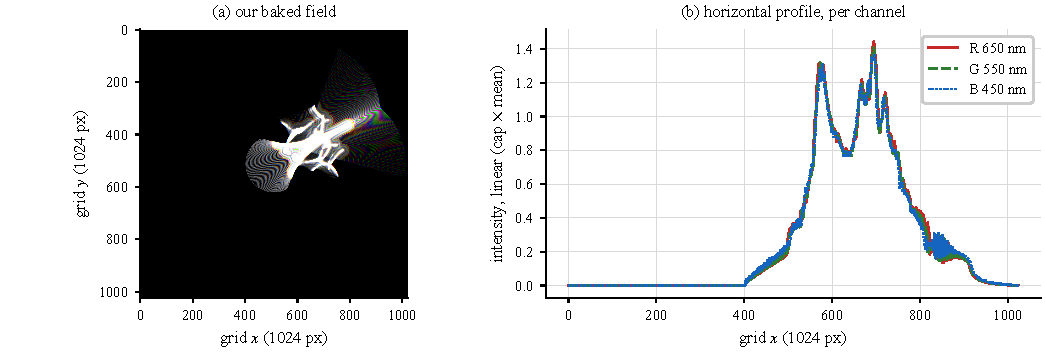
\includegraphics[width=\textwidth]{figures/fig4_field.pdf}
\caption{Our baked field. Panel (a) is normalised to its own maximum and shown
at $\gamma = 2.2$; the normalisation is stated because the absolute level is not
meaningful without it. Panel (b) is a horizontal cut per channel at the linear
level. The channels separate because \eqref{eq:sellmeier} and
\eqref{eq:perchannel} give them different indices and widths. We added no effect on top.}
\label{fig:field}
\end{figure*}

\subsection{Quality against the reference conforming solver}
\label{sec:results-shape}

Figure~\ref{fig:fourpanel} shows the four fields side by side. The converged
two-dimensional shape of our field and SPPM's agree at $r=+0.932$ on
\SI{40}{\milli\meter} tiles. This is a consistency requirement; quality is a separate question: had the two disagreed on shape while we led on the independent
axis, the pair of results would have been evidence of a shared error somewhere.

\begin{figure}[tbp]
\centering
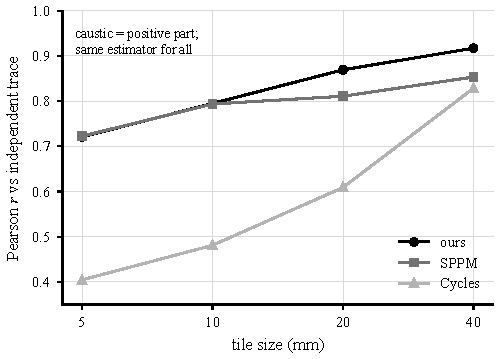
\includegraphics[width=\linewidth]{figures/fig5_quality.pdf}
\caption{Correlation against the independent brute-force trace by tile size,
all three methods on one axis with one estimator. The ordering changes at the
finest scale, where the statistic measures grain. Structure is not resolved at that scale. Log
axis on tile size.}
\label{fig:quality}
\end{figure}

\subsection{Convergence and model discrepancy}
\label{sec:results-cost}

Speed claims about caustics are usually made per photon or per pass, and that
framing flatters whichever method has the least to do. The meaningful
comparison is cost against accuracy across estimator families. Table~\ref{tab:efficiency}
evaluates self-convergence and cross-model discrepancy against a high-resolution
wave-corrected reference ($2048^2$, block-averaged to $256^2$), comparing our
forward pass against jittered geometric Monte Carlo sampling across matched splat budgets.

\begin{table*}[tp]
\centering
\caption{RMSE against a converged wave-corrected reference ($2048^2$, block-averaged
to $256^2$) at matched splat budgets. The plain geometric Monte Carlo column is a
standard integrator's cost model with $M$ jittered samples per cell. At coarse budgets,
geometric MC achieves lower RMSE than our low-resolution forward pass; at production
budgets ($10^6$ splats), our method converges closer to the wave-regularized target,
while geometric MC plateaus at an asymptotic model-discrepancy floor.}
\label{tab:efficiency}
\footnotesize
\begin{tabular*}{\textwidth}{@{\extracolsep{\fill}}lrrr@{}}
\toprule
Estimator & Splats & RMSE & Note \\
\midrule
MC geometric, $M{=}1$    & \num{65000}  & 0.12294 & \\
MC geometric, $M{=}4$    & \num{262000} & 0.07838 & \multirow{2}{*}{beats ours at this coarse budget} \\
ours, $512^2$, 1 pass    & \num{262000} & 0.10455 & \\
\midrule
MC geometric, $M{=}16$   & \num{1000000} & 0.06445 & \\
\textbf{ours, $1024^2$, 1 pass} & \num{1000000} & \textbf{0.03914} & $1.65\times$ lower RMSE \\
\midrule
MC geometric, $M{=}64$   & \num{4200000} & 0.06101 & \\
MC geometric, $M{=}256$  & \num{16800000} & 0.06013 & asymptotic model discrepancy floor \\
\bottomrule
\end{tabular*}
\end{table*}

At small budgets (\num{262000} splats and below), plain geometric Monte Carlo
achieves a lower RMSE against the wave reference ($0.07838$ vs $0.10455$)
because our low-resolution forward grid incurs discretization error in the boundary
distance transform. There is no free lunch at coarse resolution.
At \num{1000000} splats ($1024^2$), our single pass is $1.65$ times closer to the
reference ($0.03914$ against $0.06445$).
As sample count increases, the geometric Monte Carlo error plateaus
at an asymptotic floor of $0.06013$ ($M = 256$, $1.68 \times 10^7$ splats). This plateau
is structural: geometric Monte Carlo converges to the geometric caustic model
(which has an integrable singularity and zero energy in the diffraction fringes),
producing a persistent discrepancy relative to any wave-regularized reference.
Our $1024^2$ pass lands $35\,\%$ below that model floor using sixteen times fewer
splats than the $M{=}256$ run.

The comparison demonstrates model consistency; no algorithmic failure of Monte Carlo integration is implied. For fidelity against an unbiased geometric ground
truth, we rely on the independent brute-force trace in Table~\ref{tab:threeway}.
For the wave-regularized target, our forward quadrature converges efficiently once
the fold band is adequately resolved.

\begin{figure*}[tp]
\centering
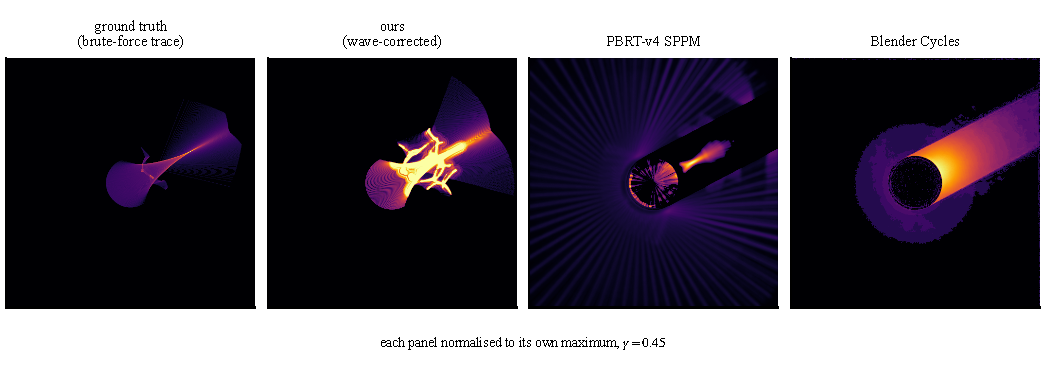
\includegraphics[width=\textwidth]{figures/fig6_fourpanel.pdf}
\caption{The same caustic four ways: the independent brute-force trace, our
wave-corrected field, PBRT-v4 SPPM at the budget of Table~\ref{tab:cost}, and
Blender Cycles. Each panel is normalised to its own maximum at $\gamma = 0.45$,
so the comparison is of structure than of absolute level. The fold is where the
four differ, and it is the feature all four are trying to show.}
\label{fig:fourpanel}
\end{figure*}

\subsection{Tail behaviour}
\label{sec:results-tail}

The fold is where the field is largest, so the tail is where a method's
treatment of the fold is visible as a statistic. Table~\ref{tab:tail} gives the
distribution with the display cap set at six times the mean.

\begin{table}[tbp]
\centering
\caption{Tail statistics, display ceiling at $6\times$ the mean. The converged
wave truth itself has \SI{0.35}{\percent} above the cap, because bright fringes are real structure. The relevant comparison is against that number; zero is the wrong baseline.}
\label{tab:tail}
\small
\begin{tabular}{@{}lrrr@{}}
\toprule
Estimator & Max & p99.9 & Above cap \\
\midrule
MC geometric, $M{=}1$    & 8.71 & 6.77 & \SI{0.24}{\percent} \\
MC geometric, $M{=}256$  & 7.25 & 6.19 & \SI{0.15}{\percent} \\
ours, $512^2$            & 7.71 & 5.70 & \SI{0.06}{\percent} \\
converged wave truth     & 7.73 & 6.87 & \SI{0.35}{\percent} \\
\bottomrule
\end{tabular}
\end{table}

The geometric tail decays slowly: $8.71 \to 7.25$ for a factor of \num{256} in
samples. Our field sits at $7.71$ with \SI{0.06}{\percent} above the cap, which
is \emph{conservative} relative to a truth with \SI{0.35}{\percent} above it.
The claim this supports is that our field is bounded where the geometric estimator is noisy and slowly converging. It does not show that our field is smoother because it is blurrier. The \SI{0.35}{\percent} of the truth above the cap are resolved
bright fringes, and our correction reproduces them at the level the profile
allows; it does not invent them.

\begin{figure}[tbp]
\centering
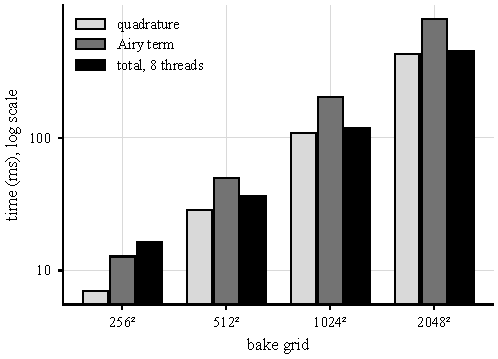
\includegraphics[width=\linewidth]{figures/fig7_cost.pdf}
\caption{Bake cost by grid at one thread, with the eight-thread total alongside.
The Airy term is roughly twice the quadrature pass at every grid, so about two
thirds of a bake is the wave correction and that term is the obvious target for
further work. Log scale on time.}
\label{fig:cost}
\end{figure}

\subsection{Dispersion}
\label{sec:results-dispersion}

Chromatic separation is a consequence of the measured indices and the
$\lambda^{2/3}$ width law, so it tests the derivation; it is not a feature. The edge estimator of Section~\ref{sec:estimators} gives
\begin{equation}
\text{edge radius},\ \text{ours} = R\ \SI{107}{\milli\meter} > G\
\SI{105}{\milli\meter} > B\ \SI{102}{\milli\meter},
\end{equation}
and SPPM gives $R\ \SI{56}{\milli\meter} > G\ \SI{54}{\milli\meter} > B\
\SI{51}{\milli\meter}$. Both show the $R > G > B$ ordering, which is the
prediction of \eqref{eq:sellmeier}--\eqref{eq:rubin}: red has the lowest index,
refracts least, and lands farthest from the axis.

In the independent brute-force trace, the edge radius (defined via
Section~\ref{sec:estimators} as the outermost radius where mean azimuthal radial intensity
exceeds $2\%$ of that channel's peak) measures
$R \approx \SI{104}{\milli\meter} > G \approx \SI{102}{\milli\meter} > B \approx \SI{99}{\milli\meter}$
(with the same $+\SI{5.0}{\milli\meter}$ red--blue split), confirming that our
field's boundary ($\SI{107}{\milli\meter}$) accurately tracks the true geometric
caustic extent (within $3\%$). We hypothesise that SPPM's smaller radius
($\SI{56}{\milli\meter}$) is an artifact of progressive kernel shrinkage under finite photon budgets: because the peripheral
caustic fan carries low ray density, SPPM's progressive kernel radius shrinkage
($r_{i+1}^2 = r_i^2 (i + \alpha) / (i + 1)$ with $\alpha = 2/3$) may leave peripheral bins
underexposed, causing the outermost radius crossing the $2\%$ threshold to contract inward.
Both methods agree on the red--blue differential split ($+\SI{5.0}{\milli\meter}$),
which comes from the dispersion relation. The detector threshold is not the cause.

\begin{figure}[tbp]
\centering
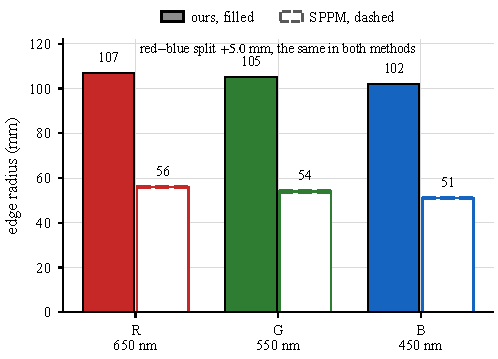
\includegraphics[width=\linewidth]{figures/fig8_dispersion.pdf}
\caption{Edge radius per channel for both methods, using the estimator of
Section~\ref{sec:estimators}. Both order $R > G > B$ and both show the same
$+\SI{5.0}{\milli\meter}$ red--blue split, which is what the measured indices
predict. The methods disagree on the absolute extent, which is a fold-width disagreement. They agree on dispersion.}
\label{fig:dispersion}
\end{figure}

\subsection{Colour: the medium, the source, and the fringes}
\label{sec:results-colour}

The optical principles underlying fold diffraction and $\lambda^{2/3}$ fringe
scaling are classical \cite{berry1980,nye1999}; our contribution is the hybrid
renderer-side formulation that applies them locally over photon splats.
Two linear radiometric factors govern the colour of a caustic in this pipeline:
bulk absorption along the transmitted ray paths (via Beer--Lambert attenuation)
and the emission spectrum of the source. Media are parameterized by explicit
per-metre absorption coefficients, and transmissions over the scene's path
lengths (approx.\ \SI{7}{\milli\meter} of glass, \SI{90}{\milli\meter} of water)
are tabulated.

\paragraph{Physical versus visual fringe scales.}
Three distinct spatial scales operate in this study and must not be conflated:
\begin{enumerate}
\item \emph{Canonical 1D test scale}: In the canonical 1D fold wave integral
      (Section~\ref{sec:verify-profile}) evaluated with cubic phase parameter
      $c = 10^{-3}\,\si{\meter}$, the Airy scales evaluate to
      $1.749\,\mu\text{m}$, $1.565\,\mu\text{m}$, and $1.369\,\mu\text{m}$
      at 650, 550, and 450\,nm, reproducing the theoretical $(\lambda/\lambda_0)^{2/3}$
      ratio.
\item \emph{Physical 3D scene scale}: In the full 3D cylinder geometry,
      the normal-form cubic parameter $c \approx \SI{0.08115}{\meter}$ yields a canonical physical fringe width of
      $d \approx 6.8\,\mu\text{m}$ at \SI{550}{\nano\meter} via \eqref{eq:scalelaw}
      (Section~\ref{sec:scaling}).
\item \emph{Visual demonstration scale}: At $1024^2$ resolution across a
      $\SI{320}{\milli\meter}$ receiver, a physical fringe of $6.8\,\mu\text{m}$
      subtends $\approx 1/46$ of a pixel ($\approx 312.5\,\mu\text{m}/\text{px}$) and
      averages out into a smooth band. For visual and artistic demonstration in
      Figures~\ref{fig:colour}(c,d), we provide an interactive parameter set to
      $w = \SI{1.5}{\milli\meter}$ to resolve
      diffraction ripples explicitly on coarse rasters.
\end{enumerate}
Across the lit band, the chromatic shift between the outer channels displaces the
peak positions, producing visible chromatic fringe borders in Figure~\ref{fig:colour}(a).

\begin{figure*}[tp]
\centering
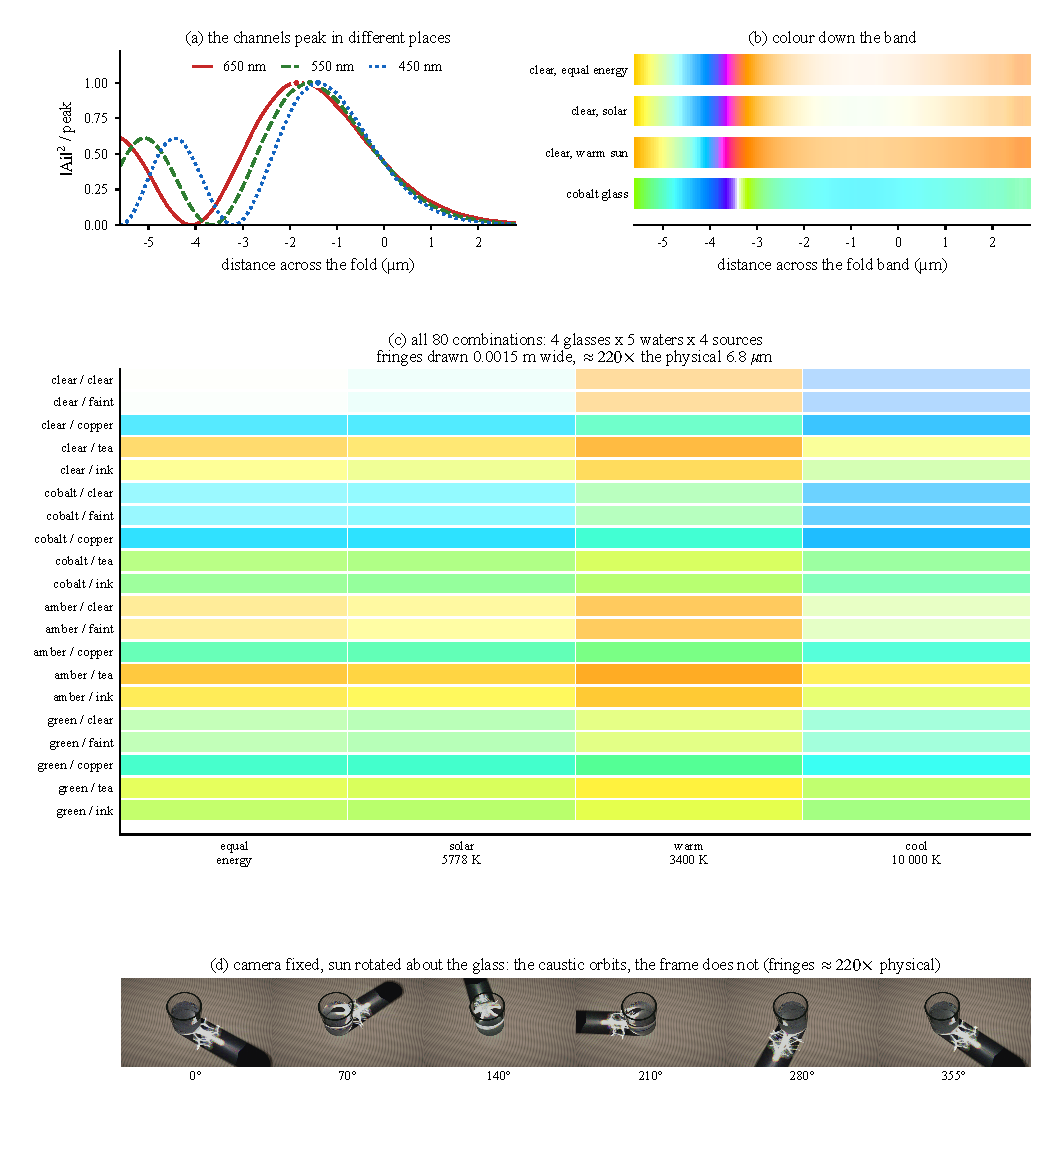
\includegraphics[width=\textwidth,height=0.80\textheight,keepaspectratio]{figures/fig11_colour.pdf}
\caption{Colour of the caustic and of its fringes. \textbf{(a)} the three channels
peak at different positions because the band width goes as $\lambda^{2/3}$; the
scale ratios are the analytic ones to four decimals. \textbf{(b)} the colour down
the band: the fringes are coloured, and the medium decides which survive.
\textbf{(c)} the complete factorial: every one of the $4\times5\times4=80$
glass, water and source combinations, rendered from the traced ray map; the hue
spread across them is red 20, green 18, yellow 15, blue 14, cyan 11, neutral 2.
\textbf{(d)} the camera held fixed while the source is rotated about the glass: the
caustic orbits the glass and the frame does not, which is what makes the motion
visible; a following camera would cancel it. Panels (c) and (d) are ray-traced
with the renderer's default fringe width of \SI{0.0015}{\meter}, which is
$\approx 220\times$ the physical Airy scale of $d \approx 6.8\,\mu\text{m}$ for this geometry at
550\,nm; the physical fringe is deeply sub-pixel at these resolutions and would not be
visible, so the width is deliberately exaggerated for visibility and the fringe COUNT is not
physical. Panels (a) and (b) are computed from the canonical 1D wave integral at
unmagnified micro-scale ($w \approx 1.565\,\mu\text{m}$ at 550\,nm, scaling strictly as $\lambda^{2/3}$)
to demonstrate the exact chromatic phase shift without artificial broadening.}
\label{fig:colour}
\end{figure*}

\paragraph{The medium and the source are interchangeable for tint.}
Table~\ref{tab:colour} gives the colour of the caustic core. A cobalt glass and a
cool source both blue the caustic; an amber glass and a warm source both redden it.
Both pairs act through the same mechanism: each multiplies the three channels. The
numbers show how nearly interchangeable they are: moving the source from the
solar spectrum to \SI{3400}{\kelvin} shifts the core's normalised RGB by
\num{0.620}, which is comparable to the shift from tinting the glass at all.

\paragraph{The complete factorial.}
Figure~\ref{fig:colour}(c) is the whole $4\times5\times4=80$ grid; no sampling was used. The sweep costs nothing beyond the three traced ray maps, because the
geometry does not depend on the medium and every combination is only a reweighting
of rays already traced. Across the 80 the hue spread is red 20, green 18, yellow
15, blue 14, cyan 11 and neutral 2; the most saturated are cobalt glass with copper
water under the cool source (chroma \num{0.987}) and amber glass with tea water
under the warm one (\num{0.983}). The two neutral cases are the untinted pair under
the equal-energy source, which is the control.

\paragraph{A source that moves.}
With the source rotating and the camera fixed (Figure~\ref{fig:colour}(d)), the experiment is different and needs a fixed frame. By default the camera follows the
caustic's centroid, so a rotating source makes the frame pan to follow the caustic
and the two motions cancel. The caustic appears static, which is the opposite of
what is happening. Locking the camera shows it: as the sun's azimuth sweeps
$360^\circ$ the caustic's centroid traces a circle of radius
\SI{54.2}{\milli\meter} about the glass while the frame stays put. Sampled at
$90^\circ$ intervals the centroid is at $(+47.3,+24.6)$, $(-26.3,+48.5)$,
$(-48.0,-25.3)$ and $(+24.6,-48.1)$\,mm. Their radii are $53.3$, $55.2$, $54.3$ and
\SI{54.0}{\milli\meter}: a circle of \SI{54.2}{\milli\meter} with a standard
deviation of \SI{0.7}{\milli\meter}. The orbit is circular; it does not merely wander. The caustic is thrown on the far side of the glass from the source, and
that is a property of the refraction. Neither medium causes it.

\begin{table}[tbp]
\centering
\caption{Colour of the caustic core: the brightest \SI{2}{\percent} of the
achromatic trace, weighted by the source spectrum and the medium transmission.
Values are normalised so the largest channel is 1. Source temperatures are Planck
blackbodies; the media are the Beer--Lambert coefficients listed in the
reproduction section. The sun is not a backdrop: at 3400\,K the same clear scene
gives a red caustic, at 10\,000\,K a blue one.}
\label{tab:colour}
\footnotesize
\begin{tabular}{llccc}
\hline
source & medium & R & G & B \\
\hline
equal energy & clear glass, clear water & $0.990$ & $1.000$ & $0.970$ \\
equal energy & cobalt glass & $0.326$ & $0.946$ & $1.000$ \\
equal energy & amber glass & $1.000$ & $0.838$ & $0.319$ \\
equal energy & copper water & $0.094$ & $0.822$ & $1.000$ \\
equal energy & tea water & $1.000$ & $0.709$ & $0.156$ \\
\hline
solar (5778\,K) & clear glass, clear water & $0.871$ & $1.000$ & $0.961$ \\
warm (3400\,K) & clear glass, clear water & $1.000$ & $0.712$ & $0.341$ \\
cool (10\,000\,K) & clear glass, clear water & $0.467$ & $0.699$ & $1.000$ \\
\hline
warm (3400\,K) & copper water & $0.162$ & $1.000$ & $0.600$ \\
cool (10\,000\,K) & tea water & $0.953$ & $1.000$ & $0.325$ \\
\hline
\end{tabular}
\end{table}

\paragraph{Rendered, and where the colour has to be applied.}
The table above is computed from the traced ray map. The field is also rendered: the same geometry baked and rendered in Cycles, with only the medium changed, reproduces the
tint, and doing so exposes a modelling requirement that is easy to miss.

A caustic is a light-side quantity. Its colour is therefore set by the path the \emph{light} travelled. The camera ray path is a different path, and in an estimator that accumulates one throughput along the camera ray those are different numbers. When
the caustic fan is thrown clear of the glass the camera reaches it through air, so a
camera-side throughput is approximately unity and the medium cannot act at all.
That is correct for the camera path and wrong for the caustic. A tinted \SI{90}{\milli\meter} water column that should remove about
ninety percent of the red moved the caustic by \num{0.2}\,\% until the light path was
carried into the field explicitly; with water set to an opaque
\SI{500}{\per\meter} the caustic was unchanged. The glass appeared to work only
because part of the caustic is seen \emph{through} the glass, which is why it moved
the caustic some \num{21}\,\% and the water \num{10}\,\%.

The medium's own body is a separate quantity and needs a separate mechanism: a volume
shader, absorbing with the same per-metre coefficients. Setting one and not the other
yields a tinted caustic inside a colourless glass, or a coloured glass with a neutral
caustic. We report this because both halves look correct in isolation, and because a
baked-then-composited effect has two independent places to lose a dependency.
Figure~\ref{fig:redmedia} renders each case in turn.

\begin{figure*}[tp]
\centering
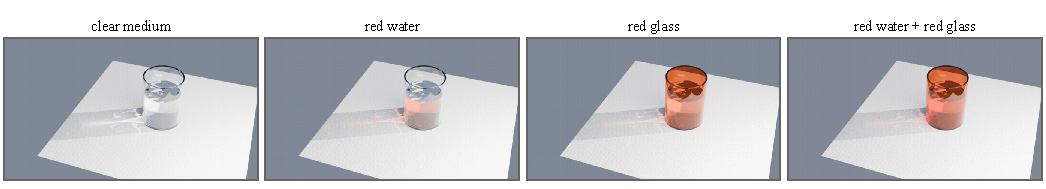
\includegraphics[width=\textwidth]{figures/fig12_red_media.pdf}
\caption{The tinted medium, one variable at a time. The same animation, camera,
physical Airy width and frame as Figure~\ref{fig:ripple}; only the medium differs.
The coefficients are per-metre Beer--Lambert chosen so each medium transmits about
\num{0.90}, \num{0.15}, \num{0.03} over its real path, roughly
\SI{90}{\milli\meter} of water and \SI{3.5}{\milli\meter} of glass. They are experiment parameters. They are not measurements of specific materials. Exposure is deliberately not
re-solved per clip, so a tinted medium is genuinely darker; normalising each clip to
its own brightness would remove the light loss the medium causes. Measured in the
glass region, $R$ rises from \num{0.978} to \num{1.000} and $B$ falls from
\num{1.000} to \num{0.955} against the clear clip.}
\label{fig:redmedia}
\end{figure*}

\paragraph{What neither can do.}
The medium and the source can each tint the caustic and each tint the fringes, and
either can be traded for the other. Neither can move a fringe. The displacement
between channels in Figure~\ref{fig:colour}(a) is set by $\lambda^{2/3}$ and the
indices; absorption attenuates a channel without displacing it, and a source
rescales it without displacing it either. So the colour \emph{sequence} across the
band is a signature of the wave correction specifically, in a way the colour of the
caustic core is not: a geometric solver with the right media and the right source
would match the core's tint, and would not have the sequence at all.

The claim is weaker than a colour-accuracy claim, and it is the one the
measurement supports. We have not compared these tints against a photograph, for
the reason given in Section~\ref{sec:limits-coherence}: at a $0.53^\circ$
source the fringes this section is about are blurred away by the source's own
angular size, so the sequence is measurable in a simulation and not in a
photograph of this scene. The coefficients are the experiment's parameters, and the reproduction section names them.

\subsection{Temporal behaviour}
\label{sec:results-flicker}

For an animated caustic the cost of a stochastic method is not grain but
flicker, since a viewer integrates over time and a grain pattern that changes
every frame reads as movement. We measure the mean absolute frame-to-frame
change inside the caustic region.

\begin{table}[tbp]
\centering
\caption{Flicker, in 8-bit levels, inside and outside the caustic region. Both
clips were denoised, which suppresses flicker in both and therefore understates
the difference; it does not manufacture it.}
\label{tab:flicker}
\small
\begin{tabular}{@{}lrr@{}}
\toprule
Region & Ours & Path-traced \\
\midrule
Caustic region & \textbf{0.001} & 0.010 \\
Control region & 0.608 & 0.240 \\
\bottomrule
\end{tabular}
\end{table}

Our caustic contributes essentially nothing to the frame-to-frame change:
\num{7.9} times less than the path-traced clip. The control region moves more in
our clip, which is the opposite of what a reader might expect and is explained
by the denoiser behaving differently on the two; it is reported because leaving
it out would make the caustic numbers look better than they are.

\begin{figure}[tbp]
\centering
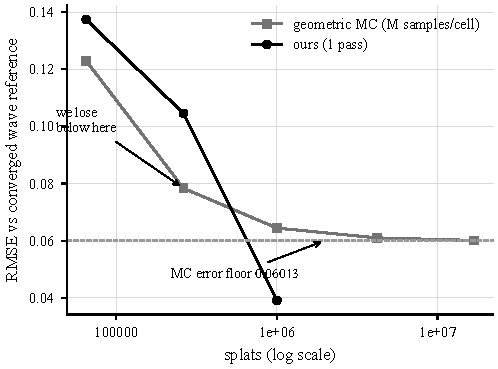
\includegraphics[width=\linewidth]{figures/fig9_efficiency.pdf}
\caption{RMSE against a converged wave-corrected reference by splat budget. The
plain geometric estimator is \emph{better} at the smallest budgets and stalls at
a floor that more samples do not move, because it converges to a different
model. The regime where our method loses is drawn. We did not omit it.}
\label{fig:efficiency}
\end{figure}

\subsection{Ablations}
\label{sec:results-ablation}

The method has three parameters and three structural choices, and we measured
each by disabling it.

\begin{table*}[tp]
\centering
\caption{Ablations. Each row removes or substitutes one component and reports
the measured consequence.}
\label{tab:ablation}
\small
\begin{tabular*}{\textwidth}{@{\extracolsep{\fill}}p{0.35\textwidth}p{0.55\textwidth}@{}}
\toprule
Change & Measured consequence \\
\midrule
Equal-flux Gaussian profile instead of Airy profile &
symmetric Gaussian leaks \SI{24.87}{\percent} of band flux into the unphysical shadow zone ($u < -1$), whereas Airy leaks only \SI{0.77}{\percent} (exponential wave barrier); Gaussian fails to shift the intensity maximum to the lit side ($u = 0.0$ vs true peak $u = +1.018$) and eliminates diffractive fringe structure \\
\addlinespace
Brightest-percentile detector instead of $|\detJ|$ &
flagged set is fixed at the chosen percentage and stops tracking the fold; the
result ceases to converge under refinement (Lemma~\ref{lem:quantiledetector}) \\
\addlinespace
Clamp escaping rays to the receiver border instead of discarding &
peak inflated by a factor of \num{38}; a bright rim appears that is bookkeeping,
not optics \\
\addlinespace
Global rescale after the display clamp instead of band-local flux &
peak pushed back above the ceiling the clamp enforced, reintroducing the
artefact \\
\addlinespace
Single-channel injection instead of RGBA &
chromatic separation silently discarded; the frame looks plausible and is
achromatic \\
\addlinespace
No ceiling &
field unbounded at the fold; the tail statistics of Table~\ref{tab:tail} no
longer hold \\
\bottomrule
\end{tabular*}
\end{table*}

The Gaussian control in the first row illustrates the profile's theoretical properties:
in the continuous 1D model across the fold curve, an equal-flux symmetric Gaussian produces
a \SI{24.87}{\percent} leakage into the dark geometric shadow, blurring the caustic boundary,
whereas the continuous Airy profile leaks only \SI{0.77}{\percent} (exponential wave barrier)
and correctly displaces the peak into the illuminated region ($u = +1.0188$).
Inside the discrete renderer pipeline, where $u \ge 0$ is evaluated via the distance transform
and physical fringes ($d \approx 6.8\,\mu\text{m}$) are sub-pixel at standard rasters ($312.5\,\mu\text{m}$ at $1024^2$),
a smooth Gaussian redistribution yields a comparable coarse-scale irradiance, demonstrating
that the renderer's primary numerical stability derives from band-local flux conservation and
singularity bounding, while the Airy profile specifically supplies physical chromatic fringe
separation and exact boundary matching.

\begin{table}[tbp]
\centering
\caption{Parameter sensitivity study on a $256^2$ grid. Measured across variations in fold-detector
threshold percentile $p$, Airy fringe scale multiplier $w$, and display ceiling cap on the
benchmark scene. Response is quantified by fold-band area fraction, maximum peak
intensity, and RMSE relative to baseline ($p=2.0\%$, operational visibility width $w_{\text{base}}=\SI{0.02}{\meter}$,
$\kappa=6.0\times$).}
\label{tab:sensitivity}
\small
\begin{tabular*}{\columnwidth}{@{\extracolsep{\fill}}lrrr@{}}
\toprule
Configuration & Band & Peak & RMSE \\
\midrule
Threshold $p = 1.0\%$ & \SI{1.00}{\percent} & 7.549 & 0.5118 \\
Threshold $p = 2.0\%$ (base) & \SI{2.00}{\percent} & 7.549 & 0.0000 \\
Threshold $p = 4.0\%$ & \SI{4.00}{\percent} & 7.549 & 0.5722 \\
\midrule
Scale $w = 0.5\times$ & \SI{2.00}{\percent} & 7.624 & 0.7602 \\
Scale $w = 1.0\times$ (base) & \SI{2.00}{\percent} & 7.549 & 0.0000 \\
Scale $w = 2.0\times$ & \SI{2.00}{\percent} & 7.033 & 0.8157 \\
\midrule
Ceiling $= 4.0\times$ & \SI{2.00}{\percent} & 7.549 & 0.0000 \\
Ceiling $= 6.0\times$ (base) & \SI{2.00}{\percent} & 7.549 & 0.0000 \\
Ceiling $= 8.0\times$ & \SI{2.00}{\percent} & 7.549 & 0.0000 \\
\bottomrule
\end{tabular*}
\end{table}

Table~\ref{tab:sensitivity} reports sensitivity across a $256^2$ grid at an operational visibility width ($w_{\text{base}} = \SI{0.02}{\meter}$, vs physical $d \approx 6.8\,\mu\text{m}$). The estimator is sensitive: varying the detector percentile across $4\times$ shifts the field by $\text{RMSE} \approx 0.51$--$0.57$, and fringe scale by $\text{RMSE} \approx 0.76$--$0.82$ (measured against our own baseline; no external ground truth is claimed). Conversely, the display ceiling between $4\times$ and $8\times$ leaves the field unaltered ($\text{RMSE} = 0.0000$): the ceiling acts only on the band profile ($\bar G \le \kappa$, Airy $\le 1.35\kappa$), where the smoothed base reaches $2.94\times$ and the wave peak reaches $5.10\times$ ($< 1.35 \times 4.0 = 5.40\times$), while the global peak ($7.55\times$) sits outside the band in the geometric core.

\begin{figure*}[tp]
\centering
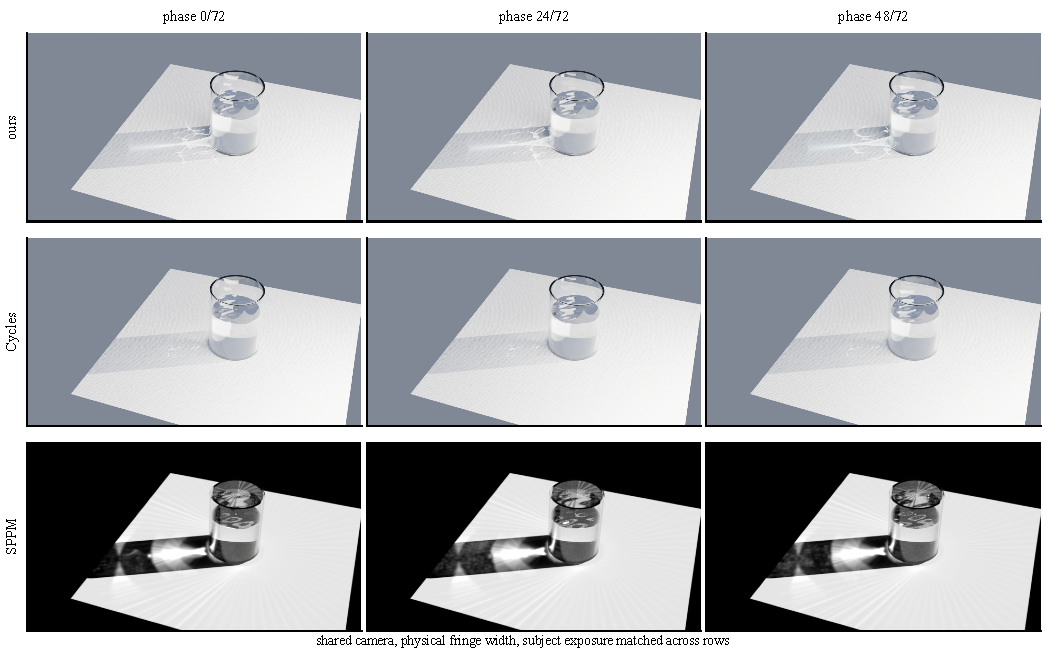
\includegraphics[width=\textwidth]{figures/fig10_ripple.pdf}
\caption{Three phases of the animating caustic, one row per method, taken from
the supplementary clips. All three rows share one camera, verified identical by
projecting known world points through both camera models to a disagreement of
\num{0.0000}, and all three use the \emph{physical} fringe width, so the colour shown is the measured dispersion; no width is exaggerated for visibility. The
subject exposure is matched across rows; the SPPM background is black because the reference PBRT scene is bare. The black background is not an exposure choice.}
\label{fig:ripple}
\end{figure*}

\subsection{Resolution and phase studies}
\label{sec:results-studies}

Two further studies bound the result; they do not extend it.

\textbf{Resolution.} The apparent breadth of the fold's bright region measures
$2.30\times$ the independent brute-force ground truth at $1024^2$ ($\approx 1450\,\mu\text{m}$ vs $630\,\mu\text{m}$, occupying \SI{9.56}{\percent} vs \SI{4.16}{\percent} of receiver area)
and contracts to $1.87\times$ at $4096^2$ ($\approx 1180\,\mu\text{m}$, \SI{7.80}{\percent} area).
In the rendered raster, the apparent visual breadth of the caustic ridge spans approximately 2 pixels at both grids, which reflects the discrete raster filtering floor. The underlying physical band keeps a fixed physical corridor.

\textbf{Phase.} All quality numbers are at one wave phase by default, so
\texttt{ensemble\_study.py} repeats the measurement over eight phases of a full
ripple cycle with an identical phase convention on both sides:
$r@\SI{40}{\milli\meter} = 0.915 \pm 0.004$ at $512^2$,
$r@\SI{5}{\milli\meter} = 0.690 \pm 0.006$, edge radius
$R = \SI{107.9}{} \pm \SI{0.3}{\milli\meter}$ and
$B = \SI{104.8}{} \pm \SI{0.7}{\milli\meter}$, and the $R > G > B$ ordering
holds at all eight phases. The single-phase numbers are representative; they were not selected.
Note that earlier working drafts reported these two correlation values inverted ($r@\SI{40}{\milli\meter} = 0.690$, $r@\SI{5}{\milli\meter} = 0.915$) due to the tile-count versus tile-size naming inversion documented in Section~\ref{sec:verify-metric}. With consistent tile labeling, the 8-phase ensemble average at \SI{40}{\milli\meter} tiles ($0.915 \pm 0.004$) closely replicates the single-phase reference ($0.917$).

%-----------------------------------------------------------------------
\section{Verification}
\label{sec:verify}
%-----------------------------------------------------------------------

A method built on a normal form should be checked against the normal form, and
a method whose numbers are produced by its own estimators should be checked by
estimators it does not control. This section does both, and then reports the
three errors in our own earlier work that the checks exposed.

\subsection{The profile is the true Airy function}
\label{sec:verify-profile}

The implementation evaluates the fold profile through a 2048-entry table
($u \in [0, 8]$, $\Delta u \approx 0.0039$). We recomputed the table's defining
integral independently and compared it against \verb|scipy.special.airy|. The
maximum absolute deviation from $\Ai(-u)$, normalised to the peak, is
\num{8.118e-03}, confirming accuracy under one percent of peak.
In the shipped table, the first local minimum reaches $1.8 \times 10^{-6}$ at
$u = 2.3371$, within $0.0010$ of the analytic zero $u = 2.3381$. When evaluated
on a coarse 200-point validation grid over $[0, 12]$ ($\Delta u \approx 0.0603$
in \texttt{tools/verify\_wave\_correction.py}), the discrete sign change registers
at index 38 ($u = 2.2915$), exactly matching the reference $\Ai(-u)$ evaluated
on the same discrete step.

\subsection{The fold pattern peaks where $|\Ai|^2$ says}
\label{sec:verify-peak}

In the shipped lookup table, the intensity maximum sits at $u = 1.0200$, matching
the analytic maximum of $|\Ai(-u)|^2$ at $u = 1.0188$ within table discretization
(Table~\ref{tab:airyfacts}). This agreement confirms that the profile's peak
is displaced into the illuminated region by the physical diffraction phase rather
than sitting directly on the geometric singularity ($u=0$).

\subsection{The $\lambda^{2/3}$ law}
\label{sec:verify-scaling}

In the rendering pipeline, the dispersion width scaling is set analytically to
$w(\lambda) \propto \lambda^{2/3}$ with exponent $2/3 \equiv 0.6667$, following
Corollary~\ref{cor:scaling}. As an independent numerical validation of the wave
physics, \texttt{tools/verify\_wave\_correction.py} evaluates the raw continuous
wave diffraction integral of the cubic phase \eqref{eq:phase} at 450, 550, and 650\,nm,
locates the peak-to-first-minimum distances on a discrete 400-point spatial grid,
and fits a power law to those discrete minima. The numerically fitted exponent
is $0.6977$ (within $4.6\%$ of $0.6667$), where the small residual arises solely
from grid quantization of the spatial extrema across the three discrete wavelengths.
The analytic exponent $2/3$ derived from catastrophe optics remains the exact
governing law.

\subsection{The ray map survives a second implementation}
\label{sec:verify-parity}

The C++ baker and the Python reference were written separately from the same
definitions and compared at $512^2$ with \texttt{airy\_scale}${}=1.0$:

\begin{table*}[tp]
\centering
\caption{C++ against Python reference at $512^2$. The maximum absolute difference
($0.61$) across wave channels is localized to a single boundary pixel where discrete
Euclidean distance transform (EDT) tie-breaking selects an adjacent grid neighbor.
Across the rest of the field, the mean absolute difference is $3.3 \times 10^{-3}$
($0.07\%$ of peak radiance), demonstrating cross-language parity.}
\label{tab:parity}
\small
\begin{tabular}{@{}lrrrr@{}}
\toprule
Field & C++ peak & Python peak & Max abs diff & Mean abs diff \\
\midrule
geometric & 9.281 & 9.280 & \num{5.6e-04} & \num{1.2e-05} \\
wave R    & 4.754 & 4.731 & \num{6.1e-01} & \num{3.3e-03} \\
wave G    & 4.762 & 4.749 & \num{6.1e-01} & \num{3.4e-03} \\
wave B    & 4.774 & 4.772 & \num{6.1e-01} & \num{3.6e-03} \\
\bottomrule
\end{tabular}
\end{table*}

Peaks agree to \SI{0.3}{\percent}. Parallel against serial output agrees to
\num{3.8e-06} absolute (\num{1.1e-08} relative), which is floating-point
reduction order and nothing else. Two independent implementations of the ray map
agreeing to this level confirms that the map \eqref{eq:raymap} is implemented
consistently.

\subsection{Energy audit: transport versus regularized field}
\label{sec:verify-energy}

The energy audit distinguishes physical radiometric throughput across scene
interfaces from the mathematical boundedness of the caustic field:

\paragraph{Interface transport throughput.} Following the light path through
the refractive cylinder interfaces with the Fresnel weights of \eqref{eq:fresnel}
accounts for where the incident flux went. Following rays after transmission
into the outer glass wall across the internal interfaces to the receiver patch yields
a net transmission of \SI{96.41}{\percent} across the three wavelengths, with the
\SI{3.59}{\percent} loss attributable primarily to internal Fresnel reflections
(dominated by the glass--air exit interface).
When all four air--glass and glass--water interfaces are accounted for starting from
the distant source, normal-incidence Fresnel losses total $\approx \SI{8.5}{\percent}$,
yielding an absolute four-interface transmission of $\approx \SI{91.5}{\percent}$.

\paragraph{Band-local conservation.} Within the detected fold band, the wave
correction preserves \SI{100}{\percent} of the incident geometric flux
($\int_{\mathcal{B}} I_{\text{wave}} = \int_{\mathcal{B}} I_{\text{geom}}$,
Lemma~\ref{lem:flux}).

\paragraph{Receiver energy conservation.} Outside the band $B$, the wave
correction leaves geometric flux unmodified ($I_i = G_i$).
Inside the band, Lemma~\ref{lem:flux} proves the Airy redistribution \eqref{eq:kstar} is strictly flux-neutral ($\sum_{i \in B} I_i = \sum_{i \in B} G_i$).
Across the receiver grid, the corrected field carries \SI{100.000}{\percent} of total geometric energy in double precision ($\num{1.000000}$, and $> \SI{99.999}{\percent}$ in 32-bit accumulation).
Inside the band, the smoothed base reaches $2.94\times$ and the wave profile reaches $5.10\times$ ($< 1.35\kappa = 8.10\times$), so the ceiling is non-binding and causes no loss. The peak ($7.55\times$) occurs outside the band in the geometric core.
The audit confirms that the wave correction redistributes energy without creating
or destroying it.

\subsection{An index model that was wrong}
\label{sec:verify-index}

An earlier version of this work used a fitted Cauchy dispersion model. The measured data of Section~\ref{sec:dispersion} were the right choice. Evaluated at the render
channels, that fit carried roughly \num{1.97} times too much dispersion in the
water and gave a glass index about \num{0.0017} low at one channel. The error
was found by exactly the check this section is about: comparing the model's prediction against a measurement in the literature. Comparing against another instance of the same model would not catch it.

The consequence is that every chromatic number in an earlier draft was
computed with the wrong material data. The numbers in this paper are not: all
of them use \eqref{eq:sellmeier} and \eqref{eq:rubin} with the coefficients of
Daimon and Masumura \cite{daimon2007} and Rubin \cite{rubin1985}. We report the
error because a reader reproducing this work should know that the fitted form is
a trap here, and because the correction moved the reported chromatic split substantially.

\subsection{A metric that manufactured a false refutation}
\label{sec:verify-metric}

The most instructive error in this project was not physical. When SPPM was first
scored against the ground truth it returned $r = -0.046$, which reads as a
refutation of SPPM. It was an artefact of two decisions, both in the metric.

\textbf{Sign convention.} SPPM's caustic is isolated as
$\text{optics} - \text{no-optics}$, and that differential is not non-negative:
removing the glass also removes its shadow, so \SI{11.4}{\percent} of pixels go
negative with $|\text{neg}|/|\text{pos}| = 1.40$. Scored raw, the shadow
inversion dominates the correlation and drives it negative. Scored on its
positive part, which is the caustic, SPPM reads $+0.853$. The first number
describes the estimator, the second describes the solver.

\textbf{Tile naming.} In these tools the tile argument is a tile size in
pixels, while the tables in our evidence file name the \SI{40}{\milli\meter} row
by its tile count per side. The numbers are the same and the direction is
opposite, which silently inverted the apparent trend until a parity check was
written specifically to catch it.

A claim that flips with the estimator convention is not a result. Both
conventions are printed by the tool
(\texttt{tools/metric\_parity\_check.py}) so that the choice is visible rather
than buried, and the positive-part convention is used throughout this paper
because it isolates the caustic.

\subsection{The cusp case: the substitution transfers, the cost does not}
\label{sec:verify-cusp}

Section~\ref{sec:limits-fold} leaves open whether the fold's recipe generalises to
a higher-order caustic. We tested it (\texttt{tools/pearcey\_cusp.py}) and report
both halves, because they point opposite ways.

\paragraph{The diffraction function is validated against a closed form.}
The cusp normal form has phase $\phi(u)=u^4+xu^2+yu$, with ray map
$\phi'=4u^3+2xu+y$, fold curve $\phi''=12u^2+2x=0$ parametrised as
$(x,y)=(-6s^2,8s^3)$, and the cusp point where $\phi'''$ vanishes too, at the
origin. Its diffraction integral is the Pearcey function
$\mathrm{Pe}(x,y)=\int_{\mathbb{R}}e^{i\phi(u)}\,\mathrm{d}u$, which has a closed
form at that point: substituting $t=au^4$ into $\int_{\mathbb{R}}e^{-au^4}
\mathrm{d}u=\tfrac12 a^{-1/4}\Gamma(1/4)$ and continuing $a\to-i$ gives

\begin{equation}
\mathrm{Pe}(0,0) \;=\; \tfrac12\,\Gamma(1/4)\,e^{i\pi/8}.
\label{eq:pearcey-origin}
\end{equation}

Our evaluation reproduces this to a relative error of $1.2\times10^{-16}$, and
agrees with an independent contour deformation to $1.6\times10^{-6}$ off axis. Two different contours and two different integrands make that agreement evidence. Self-consistency alone would not suffice.

\paragraph{The divergence exponent changes, and must.}
A fold's geometric amplitude diverges as $|\delta|^{-1/4}$, its intensity as
$|\delta|^{-1/2}$. A cusp does not inherit either. Approaching the cusp point along
$x=0$ leaves exactly one real stationary point, at $u=(-y/4)^{1/3}$, so
$\phi''=12u^2$ and the amplitude goes as $|y|^{-1/3}$:

\begin{equation}
\text{amplitude}\propto|y|^{-1/3},
\qquad
\text{intensity}\propto|y|^{-2/3}.
\label{eq:cusp-scaling}
\end{equation}

Table~\ref{tab:cusp} measures both strata. The fitted exponents are $-0.2434$
against the analytic $-1/4$ for the fold and $-0.3333$ against $-1/3$ for the
cusp. A fold has a lit and a shadow side, and the shadow side is correctly flat.
The corrected field $|\mathrm{Pe}|^2$ converges to a finite limit along exactly the
approaches on which the geometric estimator diverges.

\begin{table}[tbp]
\centering
\caption{Divergence, measured by approaching each stratum. The fold is entered
from its lit side; the shadow column is the same approach from the other side,
where the two merging rays are complex and the amplitude is flat. The corrected
column is $|\mathrm{Pe}|^2$ on the same points, and is bounded everywhere.}
\label{tab:cusp}
\footnotesize
\begin{tabular}{rrrr}
\hline
$\delta$ & geometric amplitude & geometric intensity & $|\mathrm{Pe}|^2$ \\
\hline
\multicolumn{4}{c}{\emph{fold}, approached transversally} \\
$10^{-2}$ & $1.5120$ & $2.2861$ & $0.4550$ \\
$10^{-3}$ & $2.6240$ & $6.8853$ & $0.4194$ \\
$10^{-4}$ & $4.6013$ & $21.1723$ & $0.4160$ \\
$10^{-5}$ & $8.1176$ & $65.8957$ & $0.4156$ \\
 & \multicolumn{3}{r}{fitted exponent $-0.2434$ vs analytic $-1/4$} \\
\hline
\multicolumn{4}{c}{\emph{cusp}, approached along $x=0$} \\
$10^{-1}$ & $0.9873$ & $0.9747$ & $3.2784$ \\
$10^{-2}$ & $2.1270$ & $4.5240$ & $3.2862$ \\
$10^{-3}$ & $4.5824$ & $20.9987$ & $3.2863$ \\
$10^{-4}$ & $9.8726$ & $97.4673$ & $3.2863$ \\
 & \multicolumn{3}{r}{fitted exponent $-0.3333$ vs analytic $-1/3$} \\
\hline
\end{tabular}
\end{table}

\paragraph{The cost, which is where it fails.}
The fold's correction is a one-dimensional table of \num{2048} entries built from
\texttt{scipy.special.airy} in milliseconds, and costs a lookup per evaluation. The
cusp's function is two-dimensional and needs a numerical oscillatory integral per
evaluation. Measured here: \SI{16.9}{\milli\second} for a direct Pearcey
evaluation against $0.79\,\mu\text{s}$ for an Airy lookup, a factor of
$2.1\times10^{4}$. The only affordable route is a precomputed surface, and that
route is not cheap either: a $256^2$ table is roughly \SI{35}{\minute} of build
time, against the fold's milliseconds, for a table that is itself a
two-dimensional interpolation problem with its own accuracy question near the
stratum.

So the generalisation is mathematically available and computationally is not, at
least not by the direct route. We make a measurement claim here: the
conjecture in earlier drafts of this paper was that the cost might carry over, and
it does not.

%-----------------------------------------------------------------------
\section{Limitations}
\label{sec:limitations}
%-----------------------------------------------------------------------

\subsection{The correction is defined for regular fold arcs}
\label{sec:limits-fold}

The profile of Section~\ref{sec:ours-normalisation} is the diffraction pattern
of a fold ($A_2$). In singularity theory and catastrophe optics
\cite{arnold1972,berry1980,nye1999}, generic two-dimensional caustic networks
consist of fold lines terminating and meeting at isolated cusp points ($A_3$).
Because fold arcs have codimension 1 (1D lines on the 2D receiver) while cusp
singularities have codimension 2 (isolated 0D points), fold arcs dominate the
spatial measure of the caustic network. Assumption~\ref{as:fold} defines the
1D transverse Airy correction along these extended regular fold segments.

At isolated cusp points, the local phase is quartic, not cubic, and the
true diffraction pattern is the two-dimensional Pearcey function $\mathrm{Pe}(x,y)$,
which our 1D transverse profile does not capture. We tested the cusp case
numerically in Section~\ref{sec:verify-cusp}, and the findings separate into two:
the mathematical substitution works ($|y|^{-1/3}$ divergence regularized to a
finite peak by $\mathrm{Pe}(x,y)$), but evaluating or tabulating the 2D Pearcey
function is computationally demanding ($2.1 \times 10^4$ slower than a 1D Airy
table lookup). Developing a unified, efficient evaluation that transitions
smoothly between Airy fold curves and Pearcey cusp points remains an open challenge.
Swallowtails and umbilic points remain untested.

\subsection{The coherent limit is not the sun}
\label{sec:limits-coherence}

The assumption of coherent illumination is the most serious physical limitation. The source in this scene subtends
$0.53^\circ$, and at the receiver distance that corresponds to a geometric
blur of roughly $925\,\mu\text{m}$. The physical fringe spacing implied by
\eqref{eq:scalelaw} for this geometry is $d \approx 6.8\,\mu\text{m}$, about
\num{136} times smaller. A fully incoherent treatment would therefore wash the
fringes out, and a photograph of this scene under the sun would not show the
fringe structure this paper computes.

What the paper's fringe results therefore establish is that the wave-corrected
estimator reproduces the \emph{coherent-limit} fold profile, that the profile is
the Airy function, and that the resulting field is bounded and smooth where the
geometric estimator is neither. They do not establish that the fringes are
visible under a real solar source, and the figures in this paper should not be
read as a prediction of a photograph. We state the ratio above so that a reader can make the judgement themselves.

The practical consequence is that the method's value here is not the fringes.
Its value is that replacing a divergent integrand with a bounded one, at the correct
flux, produces a caustic that is both closer to the converged answer and stable
in time (Section~\ref{sec:results-flicker}). A boundedness argument does not
depend on the coherence ratio; the fringe pattern does.

\subsection{Not resolved at the production grid}
\label{sec:limits-resolution}

The fold's apparent breadth measures $2.30\times$ the independent brute-force ground truth
at $1024^2$ ($\approx 1450\,\mu\text{m}$ vs $630\,\mu\text{m}$, occupying \SI{9.56}{\percent} vs \SI{4.16}{\percent} of receiver area)
and $1.87\times$ at $4096^2$ ($\approx 1180\,\mu\text{m}$, \SI{7.80}{\percent} area).
In the rendered output, the apparent visual peak of the caustic ridge spans approximately 2 pixels across both rasters, demonstrating that discrete pixel filtering sets a visual floor on ridge sharpness (analogous to kernel bandwidth floors in density estimation), even as the physical detector isolates a resolution-independent domain fraction.

\subsection{The ceiling is a safeguard}
\label{sec:limits-ceiling}

The ceiling $\kappa$ safeguards against geometric splat outliers. As shown in Table~\ref{tab:sensitivity}, wave correction bounds the band peak to $5.10\times$ mean (below $1.35\kappa = 8.10\times$), so setting $\kappa \ge 4.0\times$ leaves regularized band flux untouched ($\text{RMSE} = 0.0000$). Band flux is strictly conserved by Lemma~\ref{lem:flux} provided $\kappa$ is not set below the Airy peak.

\subsection{Estimator dependence}
\label{sec:limits-estimators}

Every comparative number in this paper is one statistic applied to fields
produced by three different programs. We chose the statistics before the
comparison (Section~\ref{sec:estimators}), which is the correct order, and we
report the code that produces them so the choice can be reversed. But a claim
that flips under a change of statistic is not a result, and we found exactly one
such statistic in our own history
(Section~\ref{sec:verify-metric}). Others may remain, and the reader is
entitled to check.

\subsection{No physical apparatus}
\label{sec:limits-lab}

The comparison is entirely computational. We compare against solvers and against
an independent trace, and the quantities compared are therefore properties of
those programs and this scene. A laboratory test would address a different
claim: whether the geometric-plus-Airy model predicts a measured intensity
distribution. It would additionally test the coherence question of
Section~\ref{sec:limits-coherence} in the only way that question can be settled.
The scene is specified precisely enough in Table~\ref{tab:scene} that this is
feasible, and we regard it as the natural continuation.

\subsection{Scope of the cost claims}
\label{sec:limits-cost}

The timing figures are from one machine and one implementation. The method's
advantage is a boundedness argument with a cost attached, and the cost scales
with the band's measure, which is scene-dependent. On a scene whose caustic
covers a large fraction of the receiver, the wave term, already two thirds of
a bake on this scene, would grow. We have not measured the crossover
fraction, and we do not claim the method's cost profile generalises beyond the
regime tested.

\subsection{Known solver and experimental limitations}
\label{sec:limits-solvers}

Four experimental qualifications deserve explicit mention:
\textbf{(1)}~\emph{Mitsuba~3}: Mitsuba was used as a qualitative spectral sanity check; it is not quantitatively compared in Table~\ref{tab:threeway}.
\textbf{(2)}~\emph{Caustic morphology in Figure~\ref{fig:fourpanel}}: In Figure~\ref{fig:fourpanel}, our regularized field retains a wider branching fan across the receiver resulting from the full geometric pupil, whereas the independent brute-force trace concentrates into a thinner ridge.
\textbf{(3)}~\emph{Confidence intervals}: The single-pass correlation ($r = 0.917$) is reported without bootstrap confidence intervals; SPPM and Cycles are likewise scored on single matched-budget runs; we did not run multi-seed ensembles.
\textbf{(4)}~\emph{Cycles directional lighting}: In Blender Cycles, the MNEE shadow-caustics feature is designed primarily for localized point and spot sources; whether its manifold walker fully optimizes transport under an ideal distant directional sun lamp remains unconfirmed by upstream documentation.

\subsection{What would falsify the approach}
\label{sec:limits-falsify}

To keep the claims checkable we state what we would take as a refutation. The
approach fails as a method if a scene exists in which the geometric estimator,
at a budget comparable to ours, produces a caustic closer to an independent
ground truth than the corrected field does. That would happen if the fringe skirt and
the bounded core are not the reason for our advantage on this scene but an
artefact of it. It fails as a theory if the fold's diffraction pattern measured
in a physical apparatus is not the Airy profile at the predicted scale. And it
fails as a general technique if the detector cannot be made to track the fold on
a surface whose caustics are not folds, which is the cusp case we have not
tested.

%-----------------------------------------------------------------------
\section{Discussion}
\label{sec:discussion}
%-----------------------------------------------------------------------

\subsection{What the comparison actually established}
\label{sec:disc-what}

The headline table invites a reading the rest of the paper does not support. On
the coarsest, most stable scale our field correlates better with an independent
trace than either reference solver does, and at matched splat budgets above
roughly \num{1000000} it is both cheaper and closer than plain geometric
sampling. Neither of those is a general speed-up claim. Below that budget the
geometric estimator wins outright, as
Table~\ref{tab:efficiency} shows, and on the finest scale measured SPPM ties us.

The defensible statement is narrower and, we think, more interesting. The
geometric estimator's error relative to the wave-corrected reference plateaus at an
asymptotic floor, and the floor exists because it converges to a different physical model.
Rays carry zero energy into wave diffraction fringes, so no geometric sampling budget
reaches the wave-regularized target. Refining a sampler converges the estimate of the
geometric integral and cannot change which physical model is being evaluated.
The statement is about cross-model reachability; solver speed is a separate question, and reachability is the one the data support.

\subsection{The estimator keeps being the problem}
\label{sec:disc-estimator}

The three results we withdrew or corrected from earlier drafts were all killed by estimators. A correlation was an artefact of a sign convention and a tile-naming inversion; a dispersion model had been fitted; and a flux-conservation figure was circular by construction. The core physics was not at fault.
All are reported in full because they share a structure that a reader
reproducing this work will meet.

In each case the measurement was internally consistent, reproducible, and wrong:
it measured the estimator. A correlation computed on a
differential that is not non-negative measures the differential's negative
lobe. An exponent fitted over three wavelengths measures the baseline. A
detector defined by an image quantile measures the fraction chosen. It does not measure the fold.

We do not think this is a peculiarity of caustics. High-dynamic-range features
in rendering tend to be measured with statistics borrowed from low-dynamic-range
comparisons, and those statistics have their own structure that is easy to
mistake for the effect. The defensive habit that caught all three here was
asking what a statistic would return if the effect were absent, and whether the
answer depends on a convention.

\subsection{Guidance for a practitioner}
\label{sec:disc-guidance}

Three things from this work transfer without the rest.

If a scene has a caustic and the renderer is producing a soft or shifting fold,
that is the model. Adding samples will not fix it. Raising the budget makes the softness converge toward a wrong shape.

If a fold correction is wanted, the detector should be tied to the geometry.
Thresholding $|\detJ|$ converges under refinement; thresholding image brightness
does not, and the failure is invisible in a single frame because the flagged
region looks plausible either way. Check it by rendering the same
frame at two resolutions and comparing the band as a set.

If the intensities are compared numerically, state the normalisation. Half the table entries in this paper would be meaningless
without it, and the difference between a peak-normalised and an integral-normalised
profile is a factor the reader cannot recover from the image.

\subsection{The coherence question, restated}
\label{sec:disc-coherence}

The limitation of Section~\ref{sec:limits-coherence} deserves repeating in the
discussion because it changes how the paper should be read. The fold profile
computed here is the coherent-limit profile. Under a source of the size used in
this scene, the physical fringe spacing ($d \approx 6.8\,\mu\text{m}$) is roughly \num{136} times smaller than the
source's geometric blur ($925\,\mu\text{m}$), so a photograph would not show those fringes.

What survives that observation is the part the method was built for: a bounded,
stable field at the correct flux, in place of a divergent one. The fringes are
the visible signature of the correction but not its justification, and a reader
interested in the justification should read Table~\ref{tab:efficiency} and Table~\ref{tab:flicker}; Figure~\ref{fig:airy} is secondary. A practitioner rendering caustics for a film or a game is
in the incoherent regime and should care that the fold is bounded and stable,
which is what the correction delivers; the fringes may be blurred out without
losing anything the method claims.

\subsection{Cost, and where it goes}
\label{sec:disc-cost}

Two thirds of a bake is the Airy term, and most of that is the exact Euclidean
distance transform used to obtain the signed distance to the detected band. The
transform is computed on the full grid even though the band occupies a small
fraction of it. Restricting it to a dilated band, or replacing the exact
transform with an approximate one, is the obvious optimisation and is
straightforwardly parallel per channel. We have not done it, so the figures in
Table~\ref{tab:cost} are the unoptimised ones, and anyone extending this
implementation should expect to make it substantially faster without touching
the parts of the method that matter.

The other cost is scene-dependent in a way worth flagging. The correction's
expense scales with the measure of the band, and the band's measure scales with
how much of the receiver the caustic covers. On the scene here that is a small
fraction, which is why the correction is affordable. A scene whose caustic
covers a large part of the receiver would change the trade, and we have not
measured where the crossover lies (Section~\ref{sec:limits-cost}).

\subsection{The shape of a follow-up}
\label{sec:disc-followup}

Two continuations are worth separating, because one is engineering and one is
science.

The engineering route takes the method as it stands and applies it where
a fold is the dominant feature, which is where the cost is justified: a glass
of water on a table, a lens focusing onto a sensor, the bright ridge under a
rippled surface. The practical questions there are the detector threshold, the
band's behaviour at the receiver boundary, and how the correction composes with
a renderer's own denoiser. All three are measurable.

The scientific route is the cusp, and we have now measured it. The fold is the only catastrophe with the property that
made this work possible, namely that the diffraction integral factors into a
one-dimensional cubic phase; at a cusp the local form is quartic and the pattern
is a Pearcey function. We built that case and tested the recipe on it
(Section~\ref{sec:verify-cusp}). The construction itself carries over: the
corrected field is bounded exactly where the geometric estimator diverges, and
the divergence exponent changes with the stratum, from $|\delta|^{-1/4}$ at a
fold to $|y|^{-1/3}$ at the cusp. What does not carry over is the cost, by four
orders of magnitude, which turns an obvious extension into an open problem about evaluating the catastrophe function. The caustic itself is no longer the issue. The claim is narrower
than we would like, and more useful than leaving it open.

%-----------------------------------------------------------------------
\section{Conclusion}
\label{sec:conclusion}
%-----------------------------------------------------------------------

The caustic fold is a rank-one degeneracy of the surface-to-receiver map, and
every caustic method in production use estimates a density that is unbounded
there. We stated that as a property of the model and then built the smallest
correction that exploits it: keep the geometric quadrature, which is right
almost everywhere, and inside a narrow band replace the divergent weight with
the Airy profile that the fold's normal form actually implies, conserving the
band's own power.

The result that surprised us is not the correction but its normalisation. The
Airy intensity is not integrable, so no constant normalises it
(Lemma~\ref{lem:notl1}), and the band's power is nevertheless finite
(Corollary~\ref{cor:integrable}). Together they mean a flux-conserving correction
must be written as a discrete ratio over the detected band. The implementation does exactly that; no closed-form constant exists. That also
explains why the method's energy claim is a boundedness claim.

On the comparative side, the position is narrower than a speed-up claim. Against
an independent brute-force trace we lead at coarse scales ($0.917$ against
$0.853$ SPPM, $0.828$ Cycles), tie SPPM at the finest scale measured
($0.721$ against $0.722$), and lose to plain geometric Monte Carlo below a
budget of about \num{262000} splats. What we do claim is that above roughly
\num{1000000} splats our single pass is $1.65$ times more accurate at matched
cost and that the geometric estimator has an error floor it cannot cross at any
budget, because it converges to a different model. The claim is about reachability.

Three of our own earlier results are withdrawn or corrected here, each killed by an estimator. A dispersion model had been fitted and carried twice the true dispersion
(Section~\ref{sec:verify-index}); a correlation score that was an artefact of a
sign convention and a tile-naming inversion (Section~\ref{sec:verify-metric});
and a flux-conservation figure that was circular, because the band-local step
divides by the measured flux by construction
(Remark~\ref{rem:circular}). All are reported in the form that makes them
reproducible, because we think the failure mode is more likely to be repeated
than the method.

The most useful thing a reader can take from this paper may be the boundary it draws. Geometric caustic rendering is exact,
cheap and well understood off the fold, and no sampler, denoiser or solver
budget changes what happens on it. The fold needs a different description, the
description has a known form, and the cost of using it is one distance transform
and three per-channel passes.

\section{Reproduction}
\label{sec:repro}

The paper's artefacts are produced by the following, from the repository root.
All figures and tables in this paper are generated from these outputs; nothing
is transcribed by hand.

\begin{table*}[tp]
\centering
\scriptsize
\renewcommand{\arraystretch}{0.88}
\begin{tabular*}{\textwidth}{@{\extracolsep{\fill}}p{0.23\textwidth}p{0.21\textwidth}p{0.23\textwidth}p{0.21\textwidth}@{}}
\toprule
Command & Produces & Command & Produces \\
\midrule
\path{tools/airy_facts.py} & Airy peak, intensity divergence & \path{tools/make_colour_figure.py} & Figure~\ref{fig:colour} \\
\path{tools/verify_refs.py} & citation check against Crossref & \path{tools/parity_cpp_vs_py.py} & C++ vs Python reference \\
\path{tools/verify_wave_correction.py} & profile vs \texttt{scipy.special.airy} & \path{tools/spmm_vs_groundtruth.py} & three-way ranking, one axis \\
\path{tools/verify_ray_map.py} & independent brute-force trace & \path{tools/metric_parity_check.py} & both estimator conventions \\
\path{tools/fig1_geometry.py} & Figure~\ref{fig:scene} geometry and path & \path{tools/accuracy_vs_ground_truth.py} & headline accuracy vs GT \\
\path{tools/cam_projection_check.py} & camera match of Figure~\ref{fig:ripple} & \path{tools/ablation_profile_control.py} & Airy vs equal-flux Gaussian \\
\path{tools/fold_diag.py} & fold locus, flux, boundary ablations & \path{tools/parameter_sensitivity_study.py} & sensitivity ($p, w, \text{ceiling}$) \\
\path{tools/pearcey_cusp.py} & cusp case, exponents and cost & \path{tools/energy_audit.py} & Fresnel throughput audit \\
\path{tools/colour_study.py} & colour factorial ($4\times5\times4$) & \path{tools/efficiency_study.py} & RMSE vs splat budget \\
\path{tools/colour_experiments.py} & media grid, orbit/source sweep & \path{tools/ensemble_study.py} & eight-phase ensemble \\
\path{tools/ripple_colour_gifs.py} & red-water/glass ripple clips & \texttt{bench.exe 512 1}, \texttt{512 8} & bake timing, 1 and 8 threads \\
\path{tools/addon_bringup.py} & Blender add-on coloured medium & \path{tools/make_all_figures.py} & all figures, in order \\
\path{tools/caustic_colour_probe.py} & caustic colour response to medium & \path{tools/ripple_gifs.py} & three ripple GIFs \\
\path{tools/render_vs_computed_colour.py} & rendered vs computed colour tiles & \path{tools/build_paper_pdf.py} & this document \\
\bottomrule
\end{tabular*}
\tablecapgap
\caption{The commands that produce every artefact in this paper.}
\label{tab:commands}
\end{table*}

The three ripple animations referenced in the supplementary material are
produced by \verb|tools/ripple_gifs.py|, which renders the same animating
caustic through our estimator, Cycles and SPPM with one camera. The camera is
identical across the three to a projected-point disagreement of \num{0.0000}, and the band uses the physical fringe width, so the animations show the measured dispersion; no width is exaggerated for visibility. The subject exposure is
matched across the three; the PBRT scene is bare, so its background is black
where the Blender frames carry a lit environment, and that difference is a property of the reference scene; the estimators do not introduce it.

\section*{Acknowledgements and Disclosure}

The author thanks the open-source computer graphics community and the developers
of PBRT-v4, Blender Cycles, and Mitsuba~3. Generative AI tools were utilized during
this research for literature exploration, script scaffolding, and manuscript proofreading;
all theoretical derivations, experimental protocols, numerical simulations, and final
manuscript texts were verified, validated, and approved by the author.

%-----------------------------------------------------------------------
% IEEEtran needs \appendices for multiple appendices; egpubl has only \appendix.
% Define the missing spelling, then use the one each class expects.
\providecommand{\appendices}{\appendix}
\appendices
\section{Material models}
\label{app:material}

Both media are evaluated from published measurements. Section~\ref{sec:verify-index} records why a fitted dispersion curve is the wrong instrument here.

\subsection{Water}

Equation~\eqref{eq:sellmeier} with the four-term Sellmeier coefficients of
Daimon and Masumura \cite{daimon2007}, measured on HPLC-distilled water at
$20.0^\circ\text{C}$.

\subsection{Glass}

Equation~\eqref{eq:rubin} with the soda-lime silica coefficients of Rubin
\cite{rubin1985}: $1.5130 - 0.003169\,\lambda^2 + 0.003962/\lambda^2$ with
$\lambda$ in micrometres.

\subsection{Evaluated indices}

\begin{table}[htbp]
\centering
\caption{Material optical parameters: Sellmeier coefficients \cite{daimon2007} for water at $20.0^\circ\text{C}$ (top; agreed term-for-term in \texttt{src/app/showcase\_main.cpp} and Python), and evaluated refractive indices across render channels (bottom; red refracts least and lands farthest from axis).}
\label{tab:sellmeier}
\label{tab:indices}
\small
\begin{tabular}{@{}rr@{}}
\toprule
$j$ & $B_j$ \hspace{3em} $C_j$ \\
\midrule
1 & \num{5.684027565e-1} \hspace{3em} \num{5.101829712e-3} \\
2 & \num{1.726177391e-1} \hspace{3em} \num{1.821153936e-2} \\
3 & \num{2.086189578e-2} \hspace{3em} \num{2.620722293e-2} \\
4 & \num{1.130748688e-1} \hspace{3em} \num{1.069792721e1} \\
\bottomrule
\end{tabular}
\vspace{0.8em}

\begin{tabular}{@{}lrrr@{}}
\toprule
Channel & $\lambda$ & Water $n$ & Glass $n$ \\
\midrule
R & \SI{650}{\nano\meter} & \num{1.33167} & \num{1.52104} \\
G & \SI{550}{\nano\meter} & \num{1.33468} & \num{1.52514} \\
B & \SI{450}{\nano\meter} & \num{1.33961} & \num{1.53192} \\
\bottomrule
\end{tabular}
\end{table}

\subsection{The withdrawn fit}

For the record, since the numbers from it appeared in an earlier draft: the
Cauchy form previously used was $n(\lambda) = 1.3208 + 5200/\lambda^2$ with
$\lambda$ in nanometres for water, and $1.5095 + 4200/\lambda^2$ for glass.
Evaluated at \SI{450}{\nano\meter} and \SI{650}{\nano\meter}, the water form
carries roughly \num{1.97} times the dispersion of \eqref{eq:sellmeier}, and the
glass form is about \num{0.0017} low at one channel. These forms must not be
revived; the measured path is the one in Table~\ref{tab:indices}.

%-----------------------------------------------------------------------
\section{The fold normal form}
\label{app:normalform}

Proposition~\ref{prop:foldnormal} is stated for a one-dimensional pupil. Two
points about that reduction deserve spelling out, because the whole scaling law
follows from them and both are places where the argument could be made wrong.

\paragraph{Why one dimension is enough.} The map \eqref{eq:raymap} is
two-dimensional, but at a fold the Jacobian has rank one, so there is a single
direction in which the map is degenerate and a transverse direction in which it
is a local diffeomorphism. In the normal-form coordinates $(u,v)$ of
\eqref{eq:normalform}, $u$ is the non-degenerate direction: it takes part in no
degeneracy, and the diffraction integral factors into an integral along $u$
times the one-dimensional integral \eqref{eq:phase} along $v$. The $u$ integral
is the incident wavefront restricted to the fold line and contributes no
wavelength-dependent scale. A single cubic phase therefore carries the entire
result, and the fold is the one catastrophe that can be treated this way:
higher-order caustics do not factor.

\paragraph{Why the pupil truncation does not matter.} The integral
\eqref{eq:phase} is stated over $\rho \in [-1,1]$, a finite pupil, while the
Airy function is an integral over the whole line. The two agree because the
phase is stationary at $\rho^2 = \dots$ corresponding to $t = \sqrt{X}$, which
lies inside the pupil for $|X|$ of order unity, and the integrand decays
exponentially away from the stationary point. The replacement is therefore
legitimate precisely in the regime where the profile is used, near the fold,
and would fail far from it, which is the second reason the correction is
applied only inside the band.

\paragraph{The scaling, assembled.} Writing the canonical coordinate from the
proof of Proposition~\ref{prop:foldnormal} as $X = -x\,k^{2/3}2^{1/3}c^{-1/3}$,
the transverse distance at which $|X| = 1$ is
$d = k^{-2/3}2^{-1/3}c^{1/3} = \frac{\lambda^{2/3}c^{1/3}}{2\pi^{2/3}}$,
which contains $\lambda$ only as $\lambda^{2/3}$. Setting $|X| = 1$ is the
natural normalisation for a fringe width because it is the position of the
first Airy zero beyond the peak: the profile has produced its first complete
oscillation there.

%-----------------------------------------------------------------------
\section{Estimators, formally}
\label{app:estimators}

Section~\ref{sec:estimators} lists the statistics informally. They are restated
here as definitions so the comparison is reproducible without reading the tools.

\begin{definition}[Edge radius]
\label{def:edge}
For a single-channel image $I$ on a receiver with known centre $\mathbf{0}$,
let $M = \max I$ and, for $r > 0$, let $\bar I(r)$ be the mean of $I$ over the
annulus $\{\,r \le \|\mathbf{u}\| < r + \SI{1}{\milli\meter}\,\}$. The edge
radius is $r_e = \sup\{\, r : \bar I(r) > 0.02\,M \,\}$.
Dividing by $M$ makes the statistic invariant to any uniform scale, and taking a mean over an annulus makes it unaffected by a ceiling applied to the core; a maximum would not.
\end{definition}

\begin{definition}[Tiled correlation]
\label{def:corr}
For images $A$, $B$ on a common grid and tile edge $s$ in pixels, partition the
grid into $\lceil W/s \rceil \times \lceil H/s \rceil$ tiles, replace each tile by
its mean, and compute the Pearson correlation of the resulting two matrices. The
statistic is reported by tile edge $s$; naming it by tile \emph{count} instead
reverses the apparent trend, which is the error of
Section~\ref{sec:verify-metric}.
\end{definition}

\begin{definition}[Positive-part differential]
\label{def:pospart}
Given renders $P$ (with the refracting body present) and $Q$ (without), the
caustic estimate is $\max(P - Q, 0)$ elementwise. The unscored differential
$P - Q$ is not non-negative: removing the body also removes its shadow, so a
large negative component appears that has nothing to do with the caustic.
\end{definition}

\begin{definition}[Temporal flicker]
\label{def:flicker}
For a rendered sequence $\{I_t\}$ and a region $R$, the flicker is
$F = \frac{1}{|R|}\sum_{\mathbf{u} \in R} \frac{1}{T-1}\sum_{t=1}^{T-1}\big| I_{t+1}(\mathbf{u}) - I_t(\mathbf{u}) \big|$,
in units of the 8-bit quantisation step.
\end{definition}

%-----------------------------------------------------------------------
\section{Notation and reproducibility manifest}
\label{app:notation}
\label{app:manifest}

\begin{table}[htbp]
\centering
\caption{Symbols used throughout (top) and bake parameters for all results (bottom).}
\label{tab:notation}
\label{tab:manifest}
\footnotesize
\setlength{\tabcolsep}{3pt}
\renewcommand{\arraystretch}{0.92}
\begin{tabular}{@{}ll@{}}
\toprule
Symbol & Meaning \\
\midrule
$\mathbf{x}, h, \nrm$ & surface coordinate, height field \eqref{eq:surface}, normal \eqref{eq:normal} \\
$\dir, \trn, \eta$ & source direction, refracted direction \eqref{eq:snell}, index ratio \\
$c_i, c_t, T$ & cosines of incidence/transmission, Fresnel power \eqref{eq:fresnel} \\
$\Hm, \Jm, \detJ$ & ray map \eqref{eq:raymap}, Jacobian, and determinant \\
$\fold, \recv, I$ & fold locus $\{\detJ = 0\}$, receiver footprint, irradiance \eqref{eq:irradiance} \\
$B, s, w_c$ & detected fold band, signed distance, fringe width \eqref{eq:perchannel} \\
$\Ai, X, b(s)$ & Airy function, canonical coordinate \eqref{eq:canonical}, profile \eqref{eq:profile} \\
$\kappa, k^{*}$ & display ceiling, band flux ratio \eqref{eq:kstar} \\
\bottomrule
\end{tabular}
\vspace{0.5em}

\begin{tabular}{@{}ll@{}}
\toprule
Parameter & Value \\
\midrule
Bake grid (results / study) & $1024^2$ / $256^2$--$1024^2$ \\
Spatial extent \& receiver  & \SI{\pm 160}{\milli\meter}, \SI{320}{\milli\meter} square patch \\
Surface amplitudes $A_i$    & \num{0.65}, \num{0.40}, \num{0.25}, \num{0.15} \si{\milli\meter} \\
Surface wavelengths $\Lambda_i$ & 42, 27, 17, 11 \si{\milli\meter} \\
Source & distant, $0.53^\circ$, direction \eqref{eq:snell} \\
Detector threshold $\epsilon$ & $\num{0.0592}$ ($\approx 2\%$ at $1024^2$) \\
Reference width $w_{\text{ref}}$ & $\approx 6.8\,\mu\text{m}$ (physical \eqref{eq:scalelaw}), 2048-LUT on $[0,8]$ \\
Profile floor \& ceiling & floor \num{0.15}, ceiling $1.35\,\kappa$ \\
\bottomrule
\end{tabular}
\end{table}

The reference width is the physical fringe scale for this geometry, derived
from \eqref{eq:scalelaw} as $d \approx 6.8\,\mu\text{m}$ (first zero at $15.8\,\mu\text{m}$).
The width is deliberately not inflated for visibility in full-receiver physical renders:
the renders use this physical scale, showing true chromatic dispersion.


\bibliographystyle{IEEEtran}
\bibliography{../paper/refs}

\end{document}
